% !TEX encoding = IsoLatin
\documentclass[english,a4paper,12pt]{article}
%\usepackage[english]{babel}
\usepackage{babel}
 
%Chargement des packages
\usepackage[utf8]{inputenc} % l'encodage des fichiers est utf-8, mettre [latin1] si necessaire
\usepackage[english]{babel} %le rapport est en français 
\usepackage{amsmath}
\usepackage{amsfonts}
\usepackage{amssymb}
\usepackage{graphicx} %pour afficher des images
\usepackage{float}	%pour forcer le placement des images.
\usepackage{geometry} %pour la modification des marges
\usepackage{fancyhdr} %pour modification des pieds de page
\usepackage{longtable}
\usepackage{listings}
%\usepackage{subfigure}
\usepackage{hyperref} %pour que les références soient des liens hypertextes
\usepackage[usenames,dvipsnames]{color} % pour les textes en gris
\usepackage{bm}
\usepackage{wrapfig}
\usepackage{caption}
\usepackage{subcaption}
%\usepackage{draftwatermark}
%\SetWatermarkScale{5}
\usepackage{varwidth,xcolor}

\newcommand{\authorDoc}{Prénom Nom}
\newcommand{\wvec}[1]{\ensuremath{\overrightarrow{#1}}}


 \hypersetup{
 colorlinks,
 breaklinks=true,backref,bookmarksnumbered=true,
 pdfauthor={J.Mª Goicolea},
 pdftitle={Práctica 04 - Métodos Computacionales en Ingeniería Civil}}

 \hypersetup{
 colorlinks,
 breaklinks=true,backref,bookmarksnumbered=true,
 pdfauthor={J.Mª Goicolea},
 pdftitle={Practice 04 - Computational Methods in Civil Engineering}}
 \usepackage{subfigure}


%\selectspanish
\title{\vspace*{-4ex}
	\bf\normalsize
	Computational Methods in Civil Engineering\\
	\Large
	Practice \#4, Topics 4-5.\\
	Mechanics of solids and structures: Cylindrical vault\\[3ex]
	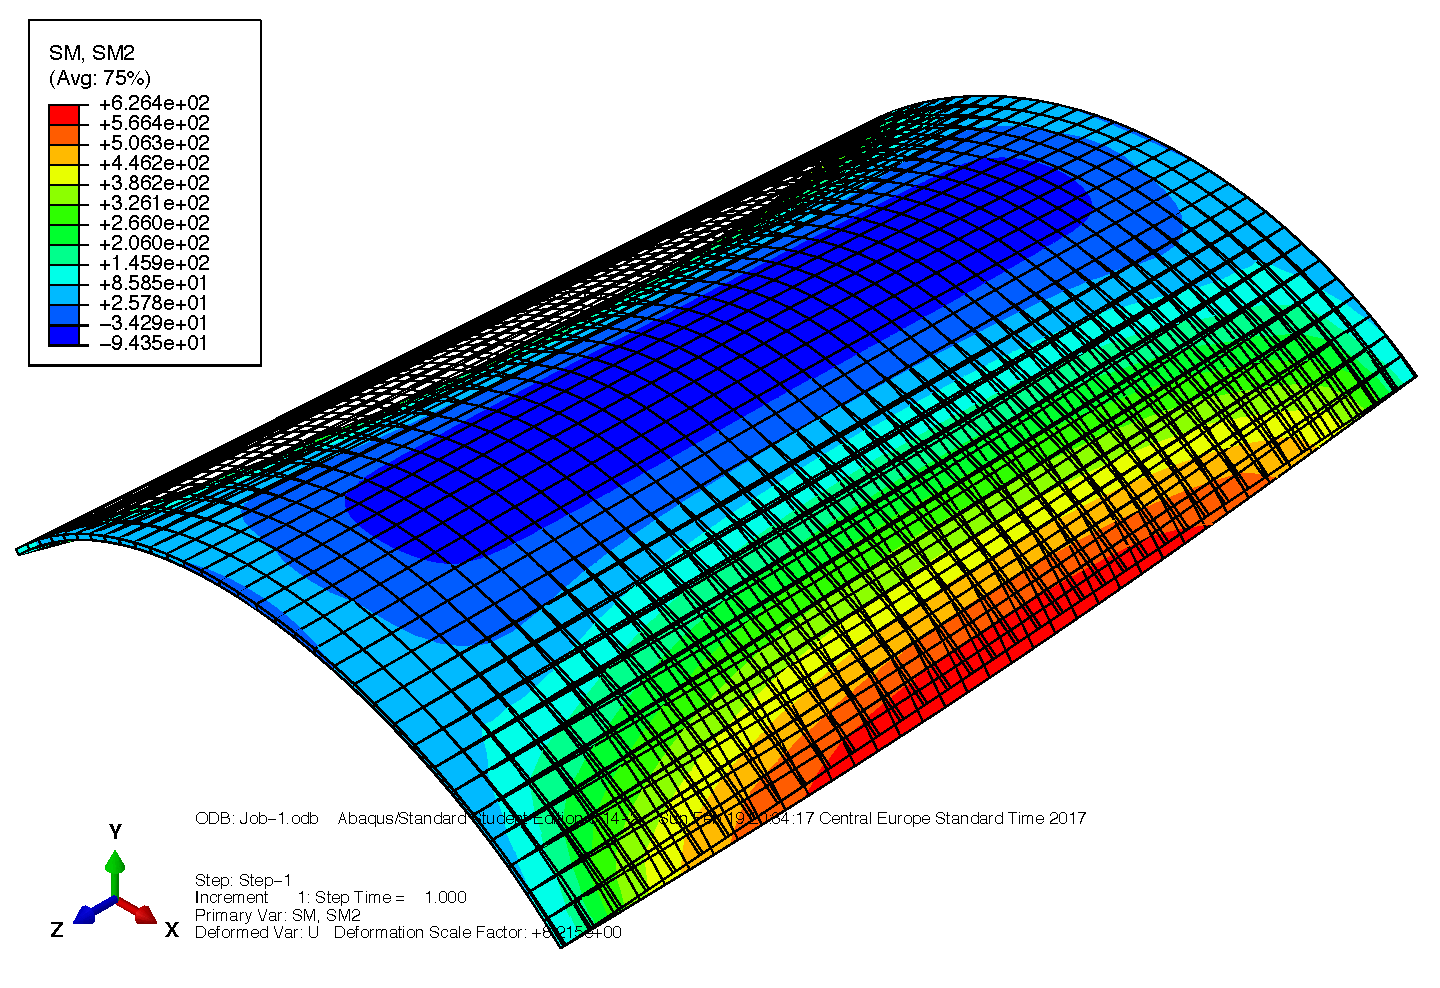
\includegraphics[scale=0.50]{figs/boveda2017-5}
	}
\author{%José M.ª Goicolea, Juan J. Arribas\\
        {\small\sc 
	Computational Mechanics Group, ETSICCP, UPM}}
\date{22-23 February 2023}


\begin{document}

\pagestyle{fancy}
\lhead[\fancyplain{}{\thepage}]{\fancyplain{}{\rightmark}}
\rhead[\fancyplain{}{\leftmark}]{\fancyplain{}{\thepage}}
\cfoot[\fancyplain{\thepage}{}]{\fancyplain{\thepage}{}}

%% \renewcommand{\chaptermark}[1]{\markboth{\sf\chaptername\ 
%%                                          \thechapter. \uppercase{#1}}{}}
\renewcommand{\sectionmark}[1]{\markright{\sf Sect.\ \thesection. #1}{}}

%\part{Métodos Generales de la Dinámica}
%\contentsline{part}{Métodos Generales de la Dinámica}{}
%\addcontentsline{toc}{part}{Métodos Generales de la Dinámica}
%\markboth{\sl Capítulo 1. Principios de la Mecánica.}{}

\maketitle

\tableofcontents

\addtocontents{toc}{\protect\hrule}

\section{Problem definition}
\label{sec:problema}
Consider a cylindrical vault roof a spanning an arch of $80^{\circ}$ 
%Se considera una cubierta en forma de bóveda cilíndrica tendiendo un arco de $80^{\circ}$ 
(Fig.~\ref{fig:esquema}).
The material is elastic with Young's modulus $E=432\,\text{MPa}$ and Poisson's ratio $\nu=0$.
%El material es elástico con módulo de Young $E=432\,\text{MPa}$ y coeficiente de Poisson $\nu=0$.
The dimensions are $R=25$ m, $L=50$ m, with thickness $t=0.25$ m.\begin{figure}[!ht]
\centering
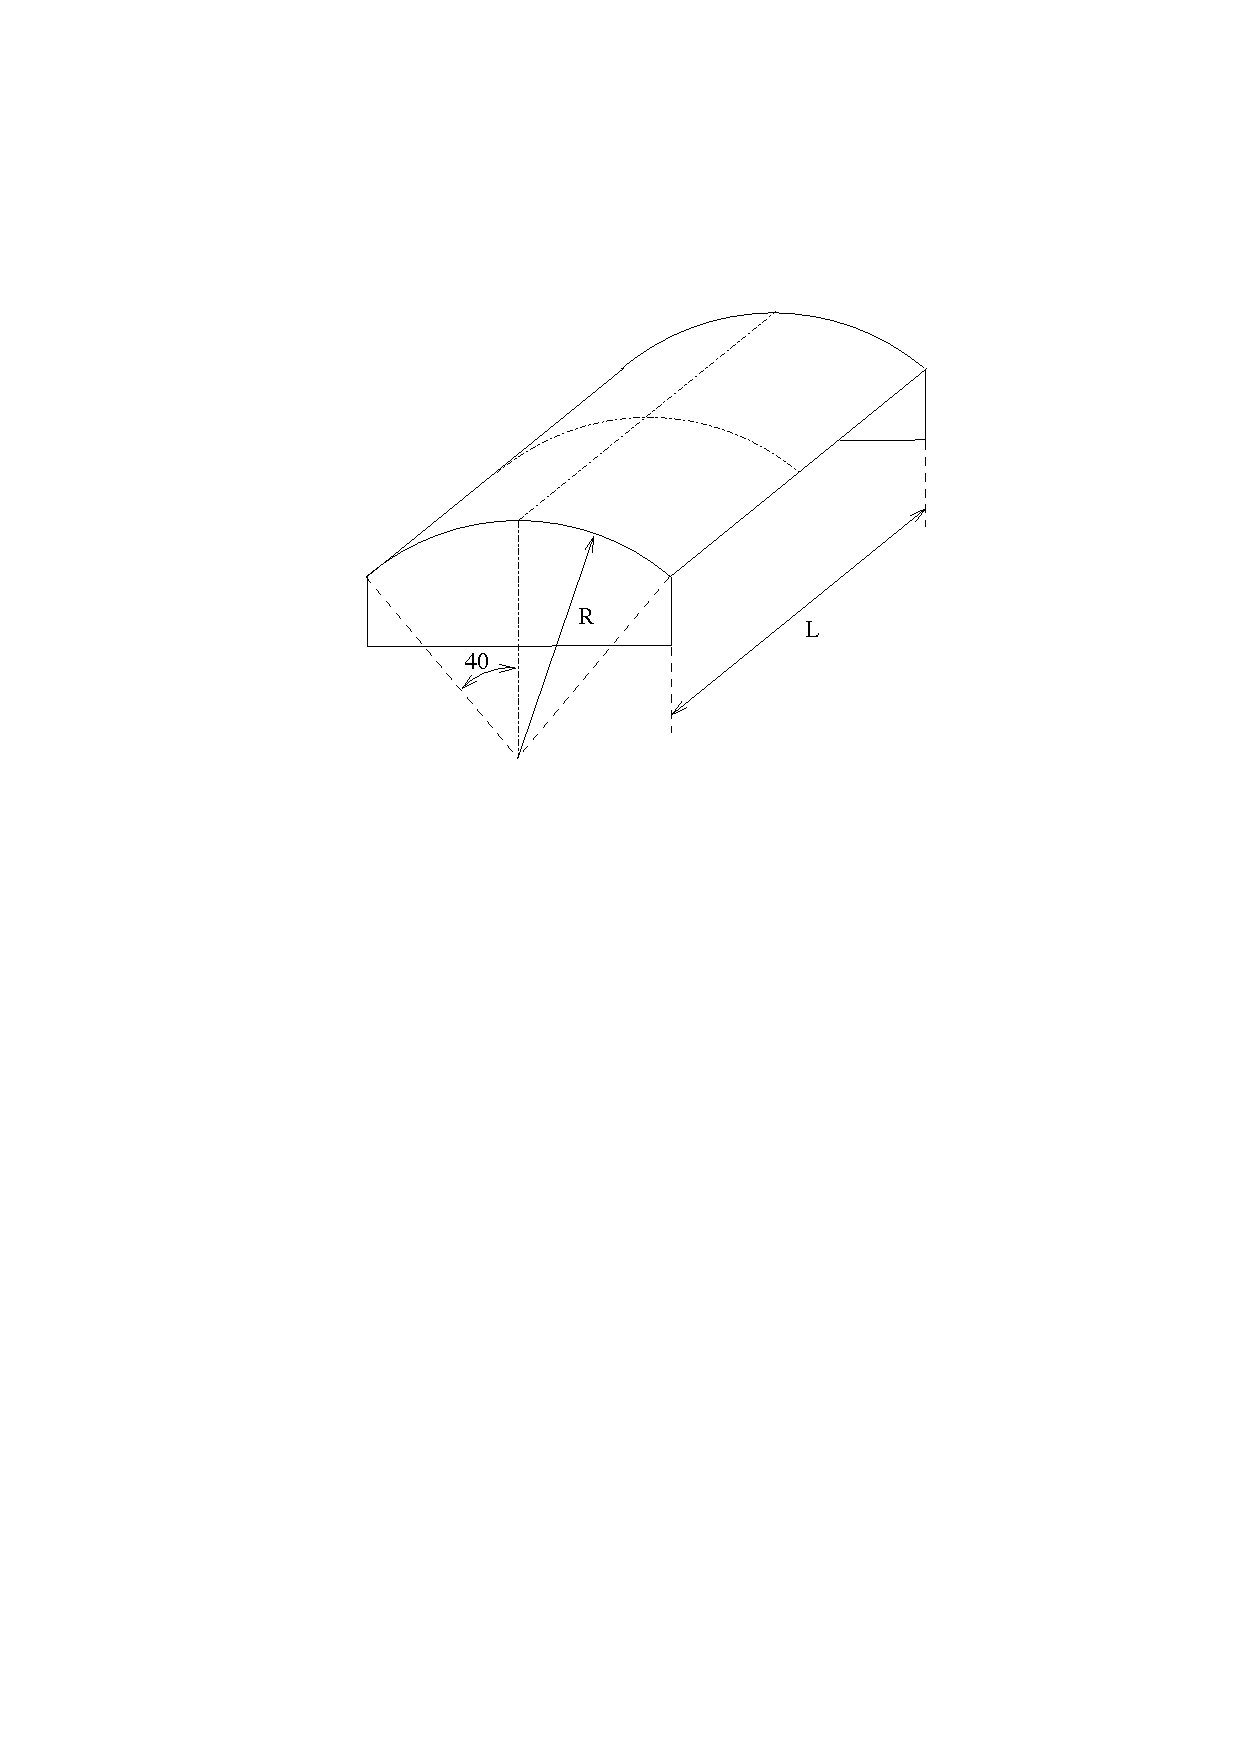
\includegraphics[width=0.5\textwidth]{figs/boveda_scordelis-lo}
\caption{Schematic definition of the cylindrical vault.}
%\caption{Definición esquemática de la bóveda cilíndrica. Las dimensiones son $R=25$ m, $L=50$ m, con espesor $t=0.25$ m.}
\label{fig:esquema}
\end{figure}

The two curved edges are simply supported on rigid diaphragms, so that the displacements both in vertical and transverse direction are constrained, and the longitudinal displacement is free.
%Los dos extremos curvos están simplemente apoyados sobre diafragmas rígidos, de forma que los desplazamientos en dirección vertical y transversal están impedidos, mientras que el desplazamiento longitudinal es libre. 
The lateral straight edges are free.
%Los bordes laterales rectos están libres. 
The roof is subject to its self-weight, with a specific weight of the material $\gamma=360\,\text{N/m}^{3}$.
%El conjunto está sometido a su propio peso, siendo el peso específico del material $\gamma=360\,\text{N/m}^{3}$.

Carry out the following tasks:
%Se pide:
\begin{enumerate}
\item
Solve the problem using 4 node shell elements with reduced integration and 5 dof per node (S4R5).
Take into account the symmetries present in the structure and loads, in order to reduce the computational model, with a mesh of $16\times 16$ elements.
%Resolver el problema con elementos lámina de 4 nodos, integración reducida y 5 gdl por nodo (S4R5), empleando una discretización de $16\times 16$ elementos. 
\item
Additionally, although a priori it may not appear to be the best approach, solve with continuum elements with the same number of surface elements and only one element in the thickness.
%Asimismo, aunque a priori no parezca la solución ideal, resolver con elementos sólidos con igual número de elementos en la superficie y un elemento tan solo en el espesor. 
Use continuum hexahedral elements of 8 nodes with full integration (C3D8), reduced integration (C3D8R) and incompatible modes (C3D8I).
%Se emplearán elementos sólidos hexaédricos de 8 nodos con integración completa (C3D8), con integración reducida (C3D8R) y con modos incompatibles (C3D8I).
\item
The results to be obtained from the analysis are the deflections in the free edge and in the top generatrix of the vault, as well as in the central section.
%Se desea obtener como resultado del cálculo los desplazamientos en el borde libre y en el borde superior de la bóveda, así como en la sección central. 
Additionally, the bending moments in the said central sections and the reactions in the diaphragms should be obtained.
%Asimismo los esfuerzos de momentos flectores en dicha sección central, y las reacciones en los diafragmas.
\end{enumerate}

\textsc{Note:} The data correspond to a classical test case for shell elements proposed by A. C. Scordelis and K. S. Lo, \emph{Computer analysis of cylindrical shells}; J. Amer. Concr. Inst 61, pp. 539-561 (1969).
%\textsc{Nota:} Se trata de un ejemplo clásico de prueba para elementos lámina propuesto por A. C. Scordelis y K. S. Lo, \emph{Computer analysis of cylindrical shells}; J. Amer. Concr. Inst 61, pp. 539-561 (1969).
The reference result which may be considered \emph{``exact''}, for the defection in the middle of the straight edge, is $0.3024$ m.
%El resultado de referencia que se puede considerar \emph{``exacto''}, para el desplazamiento vertical en el medio del borde libre, es $0.3024$ m.


\section{Model with shell elements}
\label{sec:guia}

\subsection{\texttt{Part} Module}

Start by executing \emph{Abaqus CAE} to create a new model.
%En primer lugar, se ejecuta \emph{Abaqus CAE} para crear un modelo nuevo. 
In order to create the model several numerical values of coordinates will be needed, these may be computed as indicated in Fig.~\ref{fig:python}, with the Python interpreter in the lower frame of the window.
%Para crear el modelo se van a necesitar algunos valores numéricos de coordenadas que se pueden calcular como se indica en la Fig.~\ref{fig:python}, mediante el intérprete de Python en el recuadro inferior de  la ventana.
\begin{figure}[h!tbp]
\begin{center}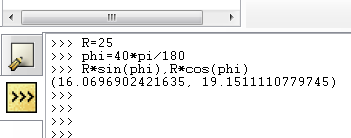
\includegraphics[scale=0.5]{capturas/01-python-calculos-aux.png}\end{center}
\caption{Auxiliary calculations for coordinates}
%\caption{Cálculos auxiliares de coordenadas}
\label{fig:python}
\end{figure}

Enter the \texttt{part} module, click the icon for creating a new part, which will be defined as 3D, deformable and shell by extrusion 
%Se entra en el módulo \texttt{part}, activando el icono de crear una nueva parte, que se define como 3D, deformable, shell por extrusión
(Fig.~\ref{fig:arco}(a)).

The model will be defined as only 1/4 of the vault, taking into account the symmetries both transverse and longitudinal.
%El modelo se definirá empleando solo 1/4 de la bóveda, haciendo uso de las simetrías longitudinal y transversal. 
First the circular line of the transverse arch is defined, selecting the icon for the utility of a circular arch with centre and 2 end points 
%En primer lugar se define la directriz circular del arco transversal, mediante la utilidad de un arco de circunferencia con centro y 2 puntos
(Fig.~\ref{fig:arco}(b)).
The centre of the circle is located at $(0,0)$, following the coordinates of the two ends of the arch ar given, for $\phi=0$ and $\phi=40^{\circ}$.
%El centro de la circunferencia se sitúa en $(0,0)$ y a continuación se dan las coordenadas de los dos extremos del arco, para $\phi=0$ y $\phi=40^{\circ}$. 
These end points to be defined are $(0,R)$ and $(R\sin\phi, R\cos\phi)$, which must be first evaluated numerically and typed in the window for point coordinates  (Fig.~\ref{fig:arco}(c)), using the dot as decimal separation.
%Estos extremos a definir son $(0,R)$ y $(R\sin\phi, R\cos\phi)$, a calcular numéricamente y escribir en la ventana de coordenadas (Fig.~\ref{fig:arco}(c)), empleando el punto como separador decimal.
When the last point (the third in this case), press the button with a red cross 
%Una vez introducido el último punto, en este caso el tercero, pulsar el botón con el aspa roja
(Fig.~\ref{fig:arco}(c)).

Make sure when generating the arch so it is created in the desired direction of the circle: for this the cursor should be located in the desired zone when the coordinates are introduced.
%\emph{OJO}: hay que tener cuidado cuando se está generando el arco para que lo haga en el sentido deseado de la circunferencia; para ello el cursor del ratón deberá estar posicionado en la zona deseada cuando se introducen las coordenadas.
\begin{figure}[h!tp]
\centering
\subfigure[Create new part]%
%\subfigure[Crear nueva parte]%
{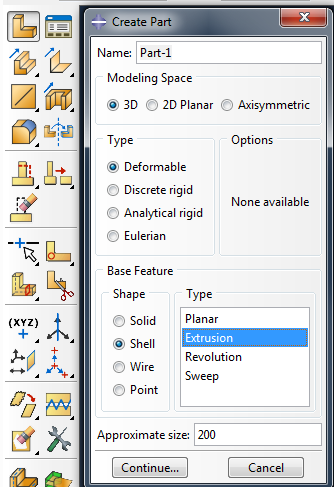
\includegraphics[scale=0.4]{capturas/02-part.png}}
\subfigure[Arch with centre and 2 points]%
%\subfigure[Arco con centro y 2 puntos]%
{\parbox[t]{0.30\textwidth}{%
\centering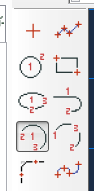
\includegraphics[scale=0.4]{capturas/03-part.png}%
}}
\subfigure[Introduction of coordinates]{
%\subfigure[Introducción de coordenadas]{
%\includegraphics[scale=0.4]{figs/01_end-coordinate-input-x}

\includegraphics[scale=0.4]{capturas/04-part}
}
\caption{Creation of the arch geometry}
%\caption{Creación de la geometría del arco}
\label{fig:arco}
\end{figure}

Once the arch is created it is accepted with the button ``Done'' (Fig.~\ref{fig:extru}(a)) and following the extrusion by a distance $L/2=25$ is performed 
%Una vez creado el arco se culmina con el botón ``Done'' (Fig.~\ref{fig:extru}(a)) y se realiza la extrusión de $L/2=25$
(Fig.~\ref{fig:extru}(b)).
After this operation we obtain a curved shell from the plane $z=0$ to the plane $z=L/2$.
The vertical planes $z=0$ and $x=0$ will be considered symmetry planes.
%Por esta operación obtendremos una lámina curva desde el plano z = 0 hasta el plano z = L/2. Los planos verticales z = 0 y x = 0 serán los considerados como planos de simetría. 
The result obtained is shown in 
%Se obtiene el resultado mostrado en la
Fig.~\ref{fig:extru1}.
\begin{figure}[h!tp]
\centering
\subfigure[select arch]%
%\subfigure[seleccionar arco]%
{
\includegraphics[scale=0.5]{capturas/05-part.png}}
\subfigure[define extrusion]%
%\subfigure[definir extrusión]%
{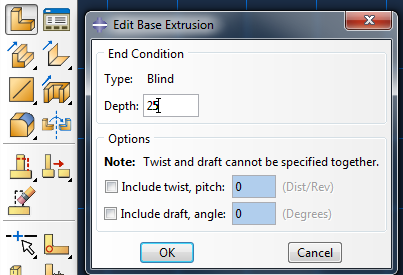
\includegraphics[scale=0.5]{capturas/06-part.png}}
\caption{Vault by extrusion of arch, between $z=0$ and $z=L/2=25$.}
%\caption{Bóveda como extrusión del arco, entre $z=0$ y $z=L/2=25$.}
\label{fig:extru}
\end{figure}
\begin{figure}[h!tp]
\centering
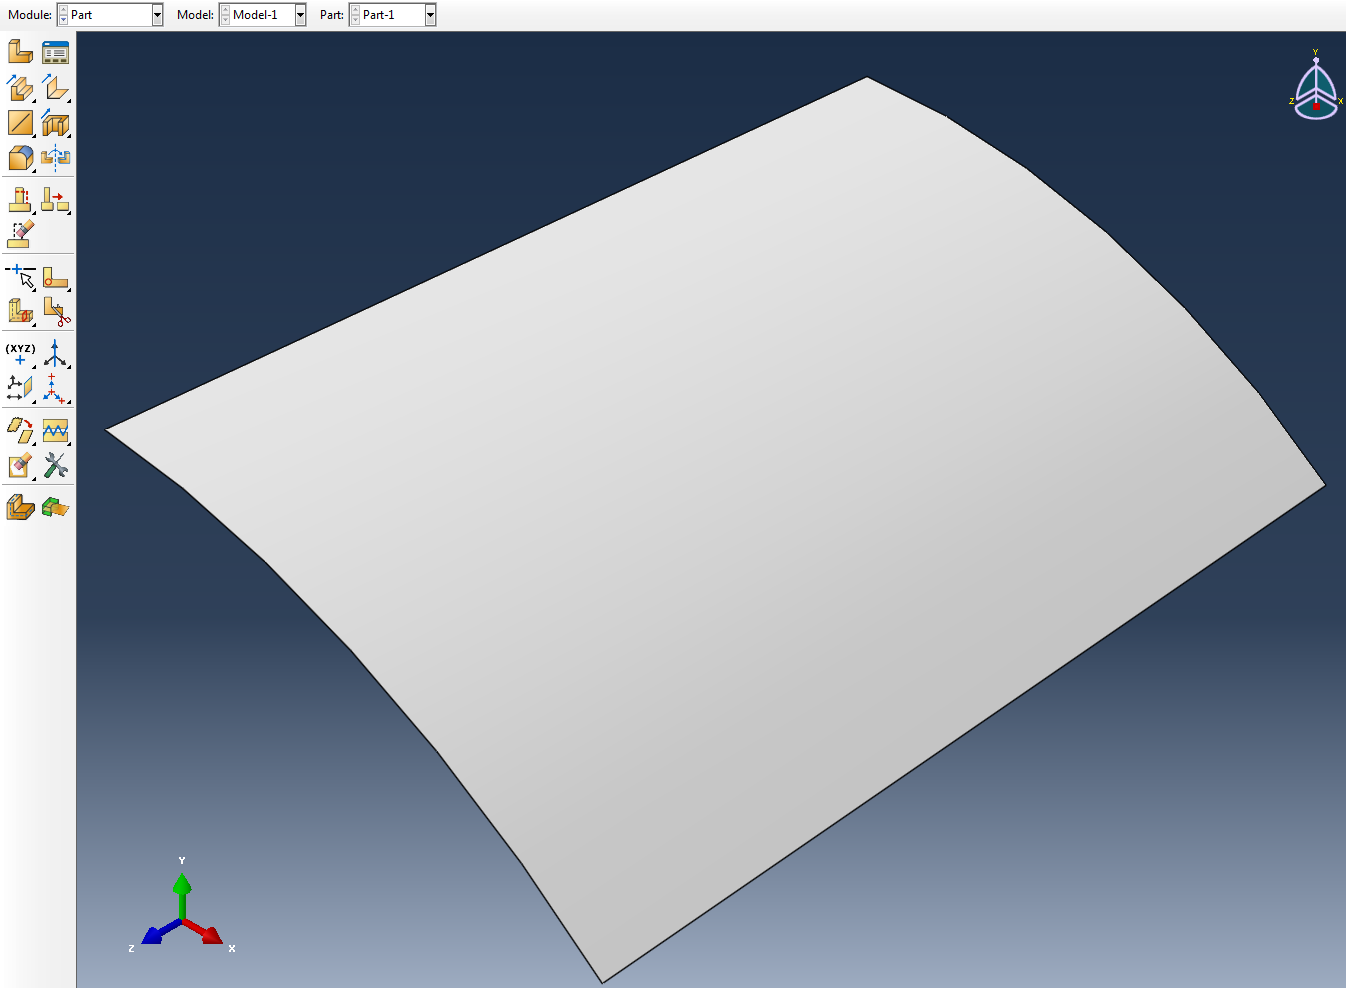
\includegraphics[scale=0.35]{capturas/07-part.png}
\caption{geometry generated for the cylindrical vault as extrusion of the arch, between $z=0$ (back side of the figure) and $z=L/2=25$ (front side).}
%\caption{Geometría generada de la bóveda cilíndrica como extrusión del arco, entre $z=0$ (parte posterior de la figura) y $z=L/2=25$ (parte anterior).}
\label{fig:extru1}
\end{figure}
\clearpage

\subsection{\texttt{Property} module}

Select the icon for creating a new material (Fig.~\ref{fig:propmat}(a)), choose a linear elastic material and type in the properties (Fig.~\ref{fig:propmat}(b)).
%Se selecciona el icono de crear material nuevo (Fig.~\ref{fig:propmat}(a)), se selecciona el material elástico lineal y se introducen las propiedades (Fig.~\ref{fig:propmat}(b)).
\begin{figure}[h!tp]
\centering
\subfigure[icon]%
%\subfigure[icono]%
{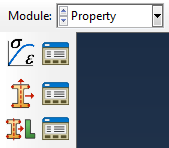
\includegraphics[scale=0.45]{capturas/08-property.png}}
\subfigure[Material type and properties]%
%\subfigure[tipo de material y propiedades]%
{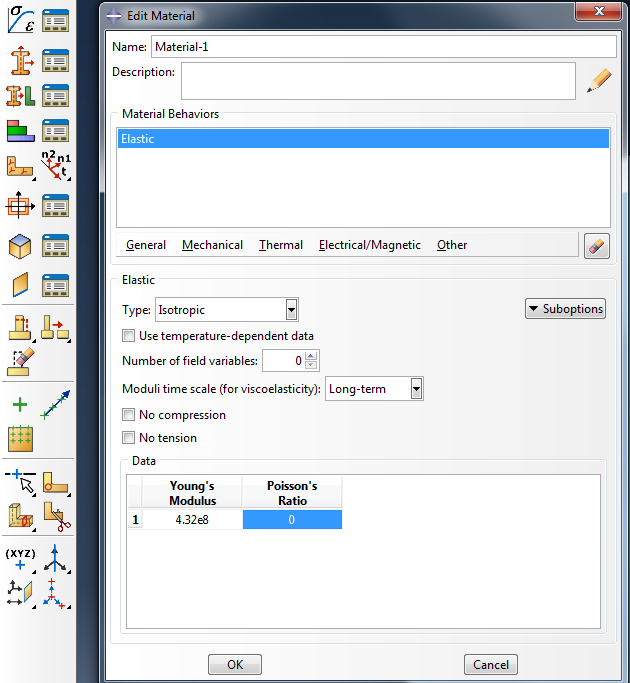
\includegraphics[scale=0.45]{capturas/09-property.png}}
\caption{Create new material}
%\caption{Crear material nuevo}
\label{fig:propmat}
\end{figure}

Following a \emph{``section''} is created, whose properties must be defined, in this case the shell thckness $(0.25\,\text{m})$ and the option \emph{``Before analysis''} (Fig.~\ref{fig:section-properties}). 
%A continuación se crea una \emph{``sección''}, en la que se definen sus propiedades, en este caso el espesor de la lámina $(0.25)$ y la opción \emph{``Before analysis''} (Fig.~\ref{fig:section-properties}). 
This option implies the shell behaviour will be computed from the section resultants (bending moments, shear forces, membrane resultants\ldots) instead of integrating numerically the stresses across the thickness, which could be necessary for a nonlinear material.
%Esta opción implica el cálculo mediante resultantes seccionales (momentos flectores, axiles\ldots), en lugar de integrar numéricamente las tensiones en el espesor, lo que podría ser necesario en un modelo de material no lineal.
Following the section is assigned to the part created previously (Fig.~\ref{fig:section-assign}).
%A continuación se asigna la sección a la parte creada (Fig.~\ref{fig:section-assign}).
\begin{figure}[h!tp]
\centering
\subfigure[type]%
%\subfigure[tipo]%
{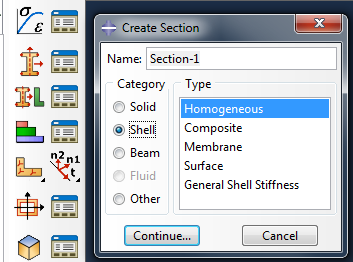
\includegraphics[scale=0.4]{capturas/10-property.png}}
\subfigure[data]{
%\subfigure[datos]{
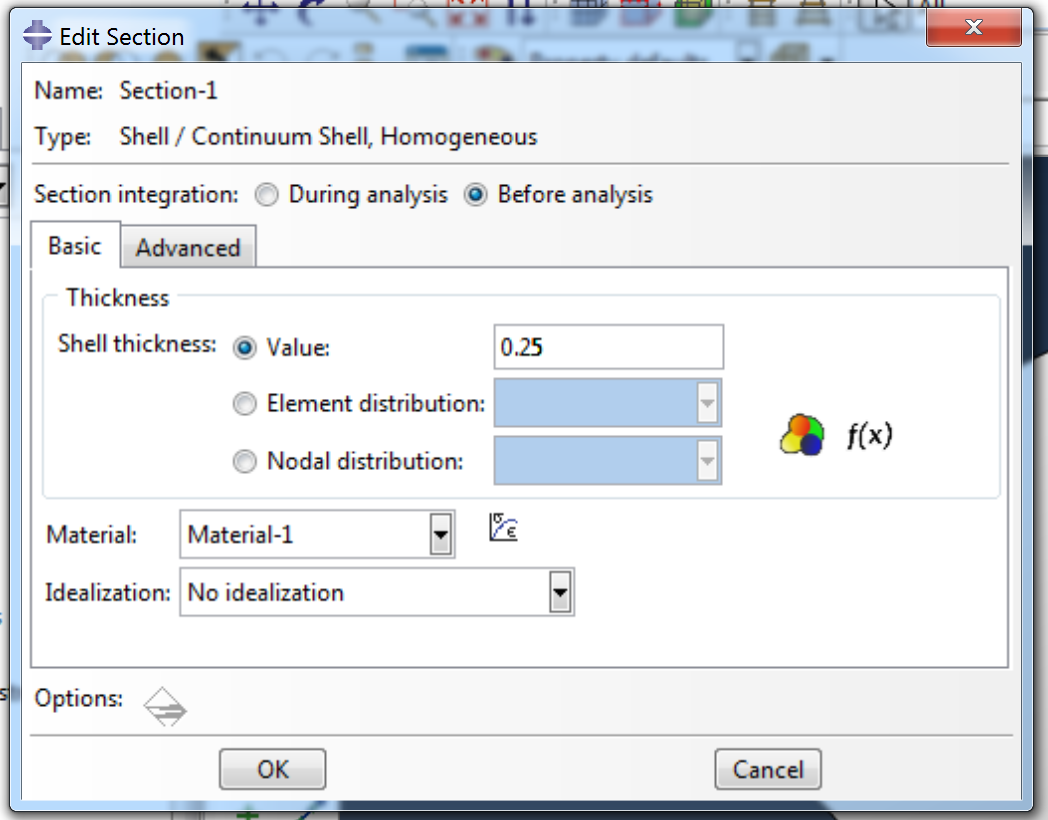
\includegraphics[scale=0.4]{capturas/02a_shell-thickness-type-selection}
%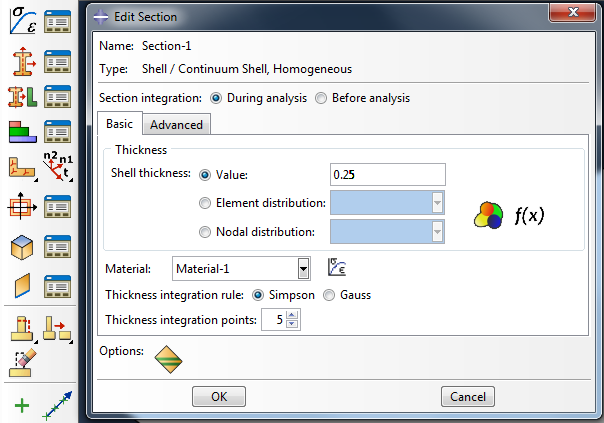
\includegraphics[scale=0.4]{capturas/11-property.png}
}
\caption{Definition and properties of the section}
%\caption{Definición y propiedades de la sección}
\label{fig:section-properties}
\end{figure}

\begin{figure}[h!tp]
\centering
\subfigure[assign section]%
%\subfigure[asignar sección]%
{\parbox[t]{0.2\textwidth}{%
\centering
\includegraphics[scale=0.6]{capturas/03a_assign-section-icon}%
}}
\subfigure[select part]{%
%\subfigure[seleccionar parte]{%
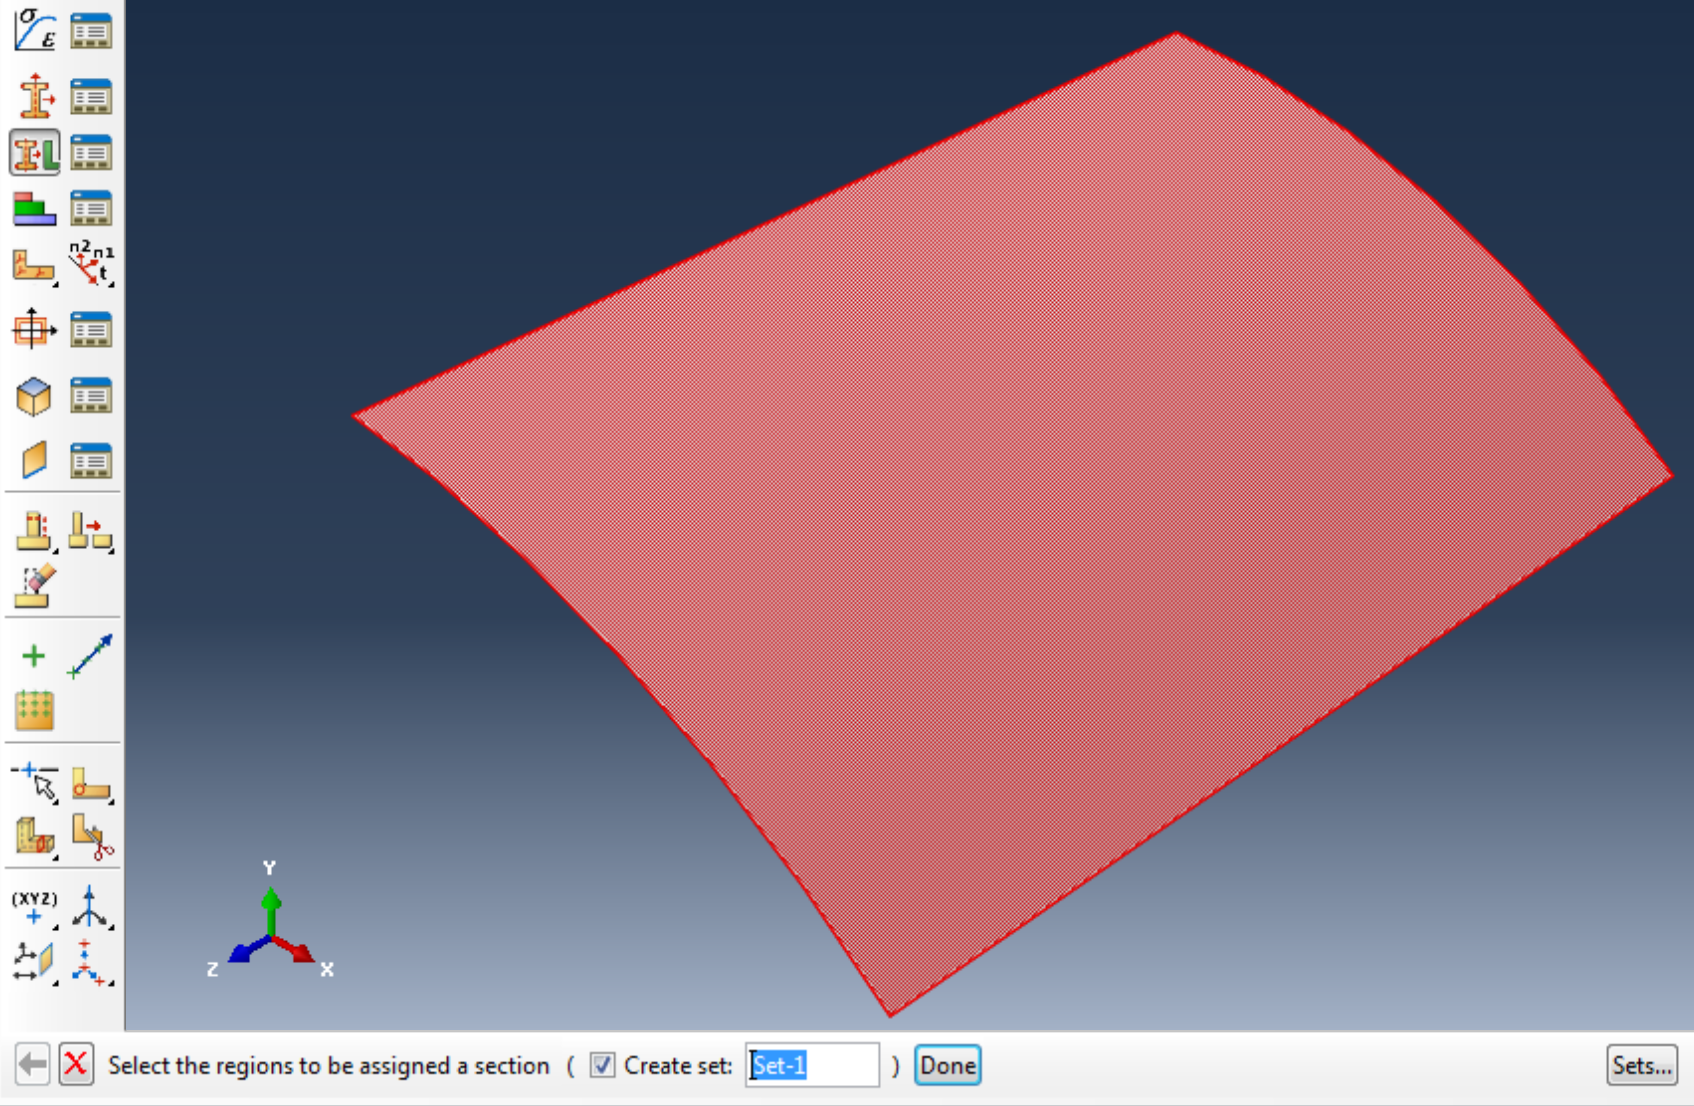
\includegraphics[scale=0.4]{capturas/04a_select-region-to-assign-section}
%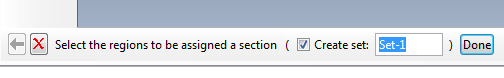
\includegraphics[scale=0.4]{capturas/12-property.png}
}
\subfigure[assignation]%
%\subfigure[asignación]%
{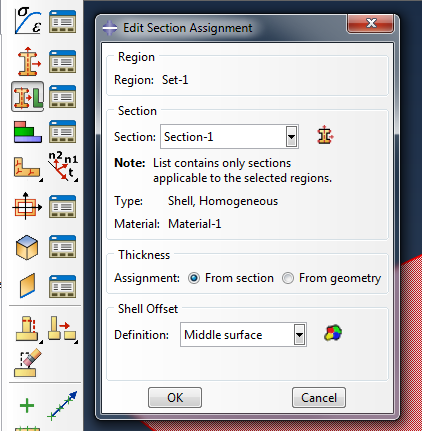
\includegraphics[scale=0.4]{capturas/13-property.png}}
\subfigure[part assigned]%
%\subfigure[parte asignada]%
{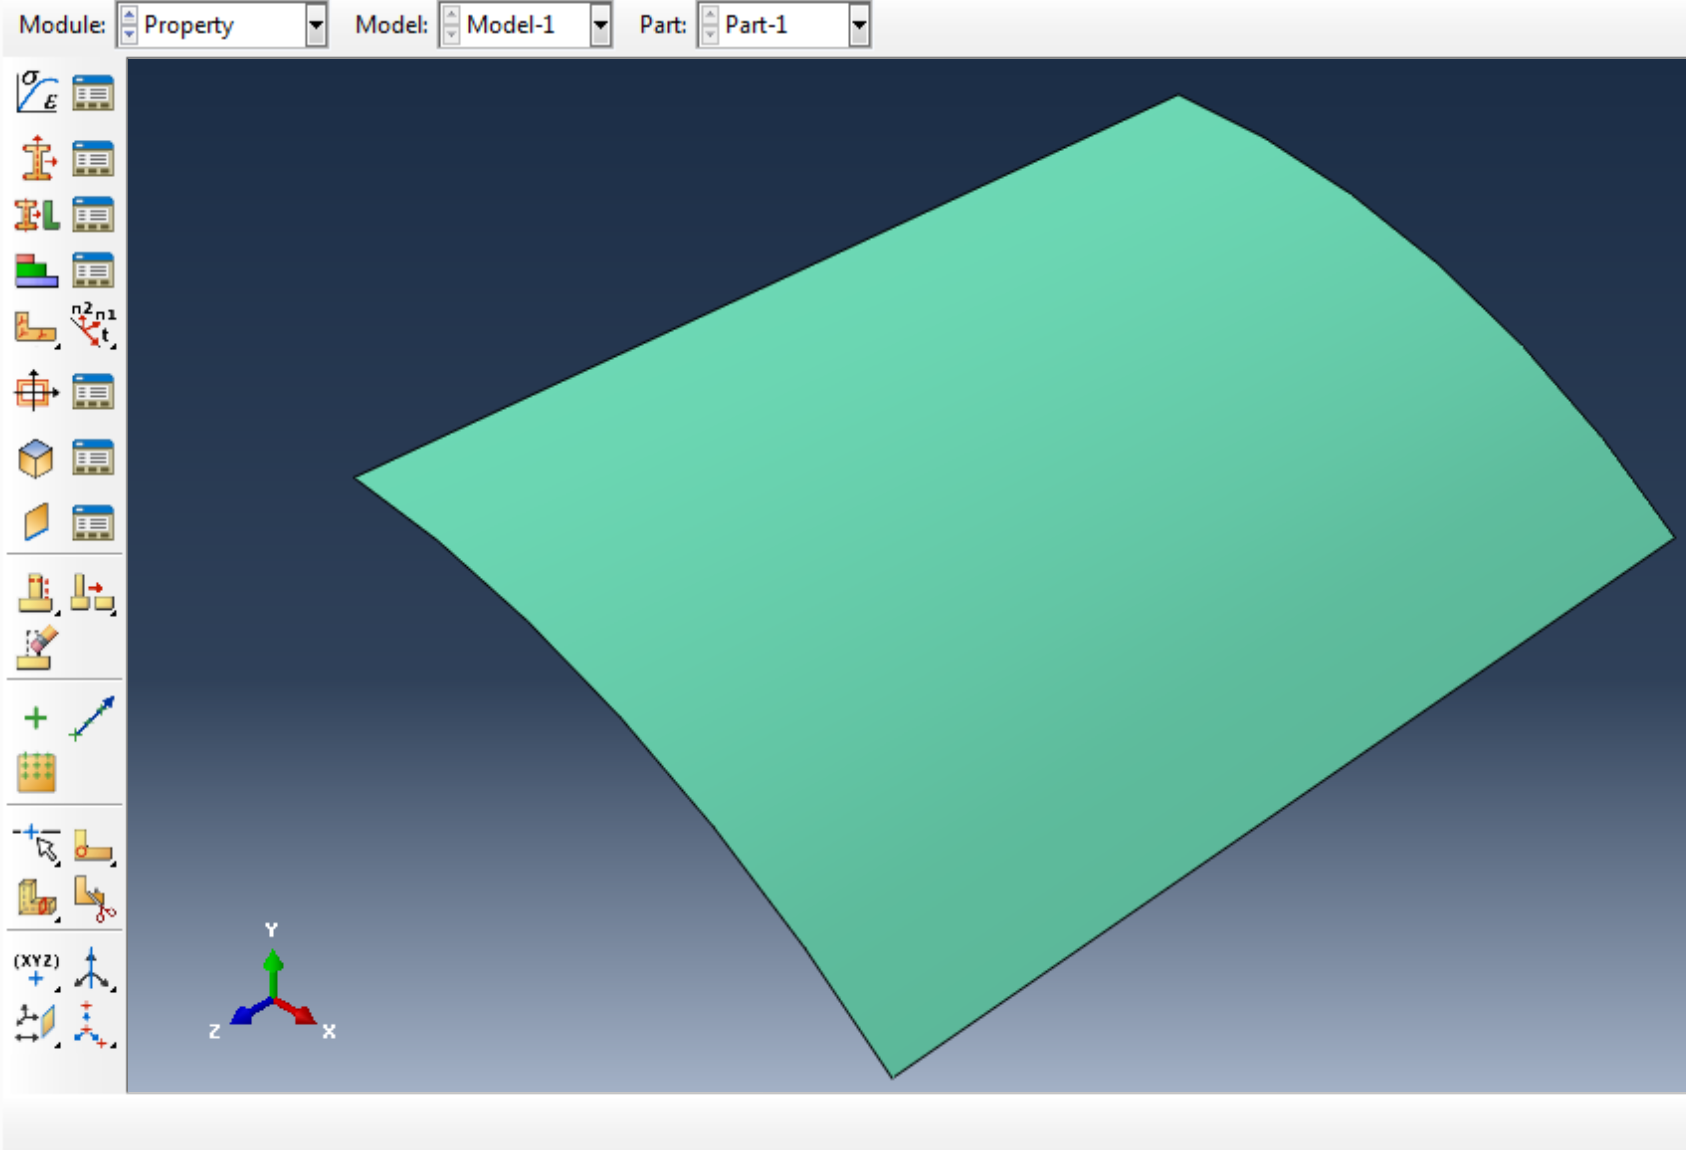
\includegraphics[scale=0.3]{capturas/05a_section-assigned}}
\caption{Assign section to part}
%\caption{Asignación de la sección}
\label{fig:section-assign}
\end{figure}
\clearpage

\subsection{\texttt{Assembly} module}

In this module one has only to create an \emph{``instance''} from the part, accepting the default options:
%En este módulo tan solo hay que crear una ``instancia'' a partir de la parte, mediante las opciones por defecto:
\begin{figure}[h!tp]
\centering
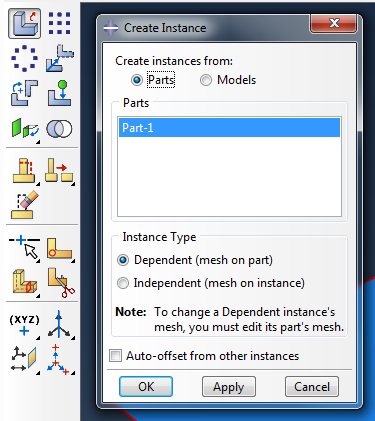
\includegraphics[scale=0.4]{capturas/14-assembly.png}
\caption{Assembly: create an instance of the part}
%\caption{Assembly: crea una instancia de la parte}
\label{fig:assembly}
\end{figure}

\subsection{\texttt{Step} module}

Now create a \emph{``step''} with the procedure type \emph{``Static, general''}.
%Se crea un \emph{``step''} para el procedimiento de cálculo \emph{``Static, general''}. 
Take the default options (Fig.~\ref{fig:step}).
%Se toman las opciones por defecto (Fig.~\ref{fig:step}). 
Within \emph{``field output''} edit the set of variables to add the section resultants SF (membrane forces and bending moments), as indicated in Fig.~\ref{fig:field-output}.
%Se edita en \emph{``field output''} el conjunto de variables para agregar los esfuerzos seccionales SF (esfuerzos de membrana y de flexión de la lámina), como se indica en la Fig.~\ref{fig:field-output}.
\begin{figure}[h!tp]
\centering
\subfigure[Creation]%
%\subfigure[Creación]%
{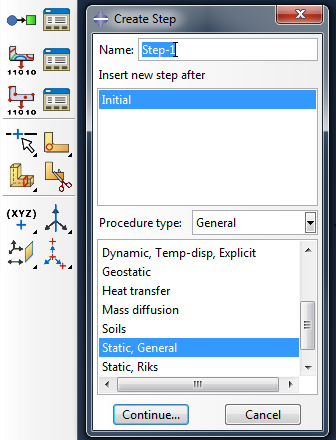
\includegraphics[scale=0.4]{capturas/15-step.png}}
\subfigure[Definition]%
%\subfigure[Definición]%
{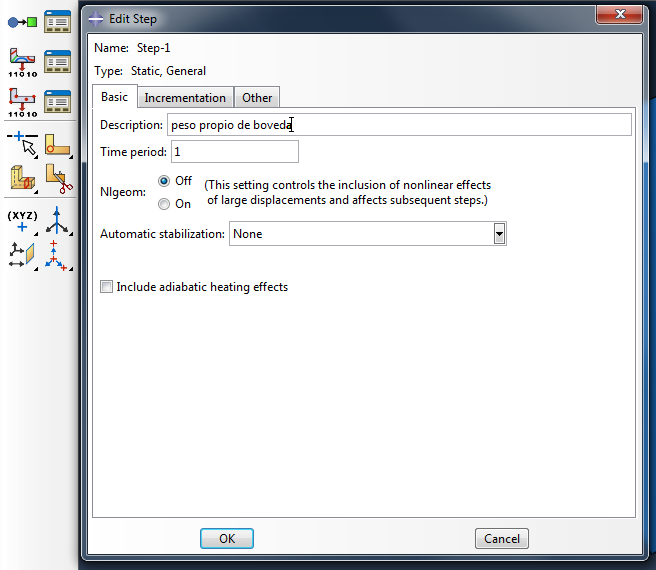
\includegraphics[scale=0.4]{capturas/16-step.png}}
\caption{Create and define the \emph{``step''}}
%\caption{Crear y definir el \emph{``step''}}
\label{fig:step}
\end{figure}
\begin{figure}[h!tp]
\centering
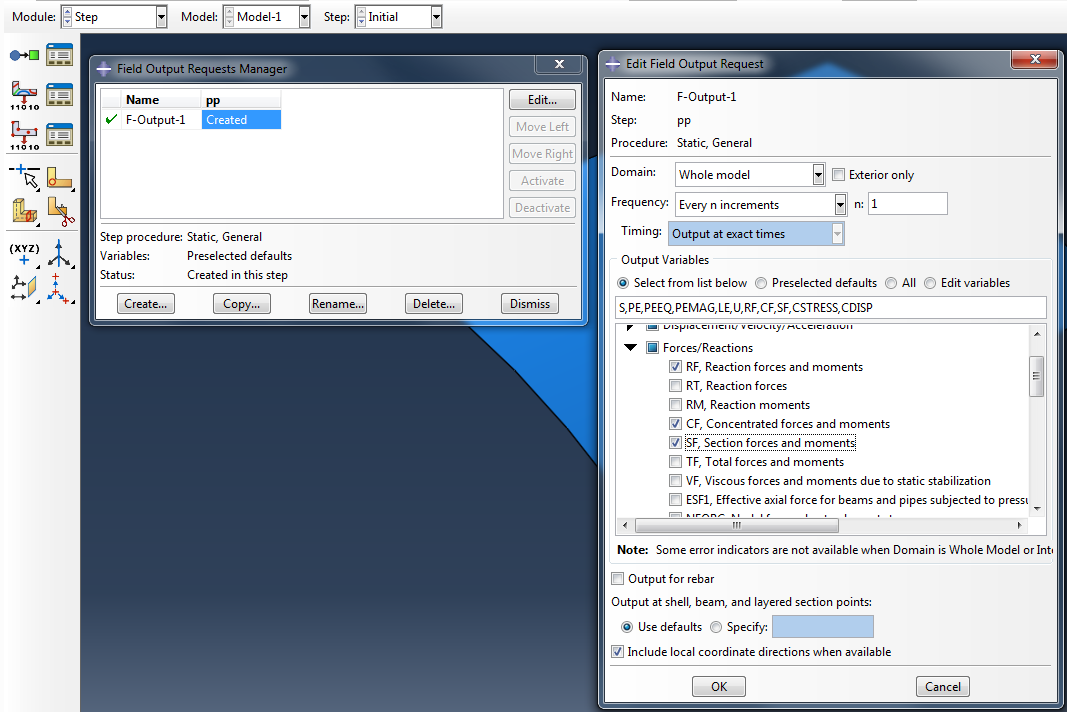
\includegraphics[scale=0.4]{capturas/16a-step.png}
\caption{Modification of the \emph{``field output''}}
%\caption{Modificación del \emph{``field output''}}
\label{fig:field-output}
\end{figure}
\clearpage

\subsection{\texttt{Load} module}

In the \texttt{Load} module both the applied loads as well as the boundary conditions will be defined.
%En el módulo \texttt{Load} se definirán las cargas aplicadas y las condiciones de contorno. 
Firt the loads are defined, these correspond only to the self-weight, through \emph{``Body force''}, assigning the value $q_{y}=-360\,\text{N/m}^{3}$ (Fig.~\ref{fig:pp}).
%En primer lugar las cargas, que son únicamente las de peso propio, mediante \emph{``Body force''}, a la que se da un valor $q_{y}=-360\,\text{N/m}^{3}$ (Fig.~\ref{fig:pp}).
The final result is shown in Fig.~\ref{fig:pp}(d).
%El resultado final se visualiza en la Fig.~\ref{fig:pp}(d)
\begin{figure}[h!tp]
\centering
\subfigure[select ``Body force'']%
%\subfigure[selecciona ``Body force'']%
{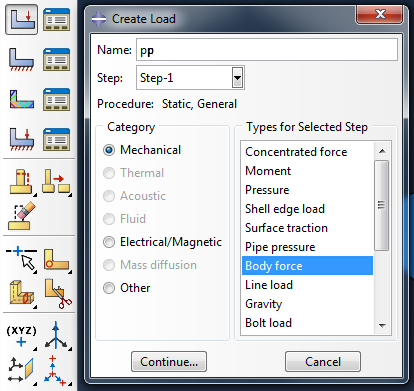
\includegraphics[scale=0.5]{capturas/17-load.png}}
\subfigure[select the body]%
%\subfigure[selecciona el cuerpo]%
{
\includegraphics[scale=0.5]{capturas/18-load.png}}
\subfigure[value of load]%
%\subfigure[valor de la carga]%
{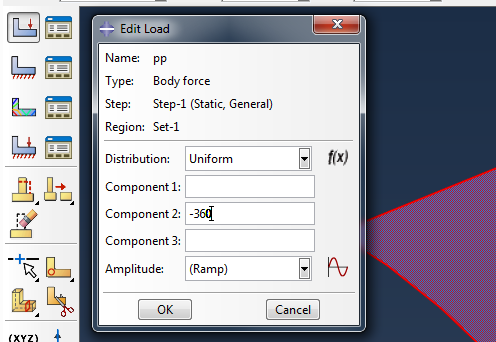
\includegraphics[scale=0.4]{capturas/19-load.png}}
\subfigure[final aspect]%
%\subfigure[aspecto final]%
{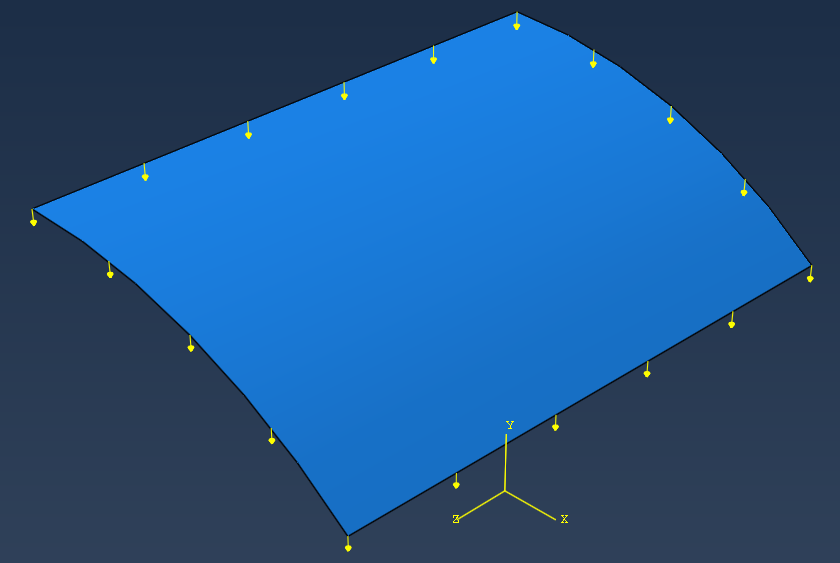
\includegraphics[scale=0.3]{capturas/20-load.png}}
\caption{Definition of self-weight loads}
%\caption{Definición de las cargas de peso propio}
\label{fig:pp}
\end{figure}

Next the boundary conditions are defined, starting by the two planes of symmetry.
%A continuación las condiciones de contorno, primero en los dos planos de simetría.
Open the \emph{``manager''} for boundary conditions and create the appropriate condition along edge $x=0$, conditions ``Symmetry/Antisymmetry'' of type ``XSYMM'', once the proper edge is selected with the mouse (watch out not to select more edges!) (Fig.~\ref{fig:xsymm}).
%Se abre el \emph{``manager''} de condiciones de contorno y se crea la condición adecuada en el borde $x=0$, condiciones ``Symmetry/Antisymmetry'' del tipo ``XSYMM'', una vez seleccionado con el ratón el borde adecuado (ojo, !`hay que tener cuidado para no seleccionar más que ese borde!) (Fig.~\ref{fig:xsymm}).
\begin{figure}[h!tp]
\centering
\subfigure[Select edge and condition XSYMM]{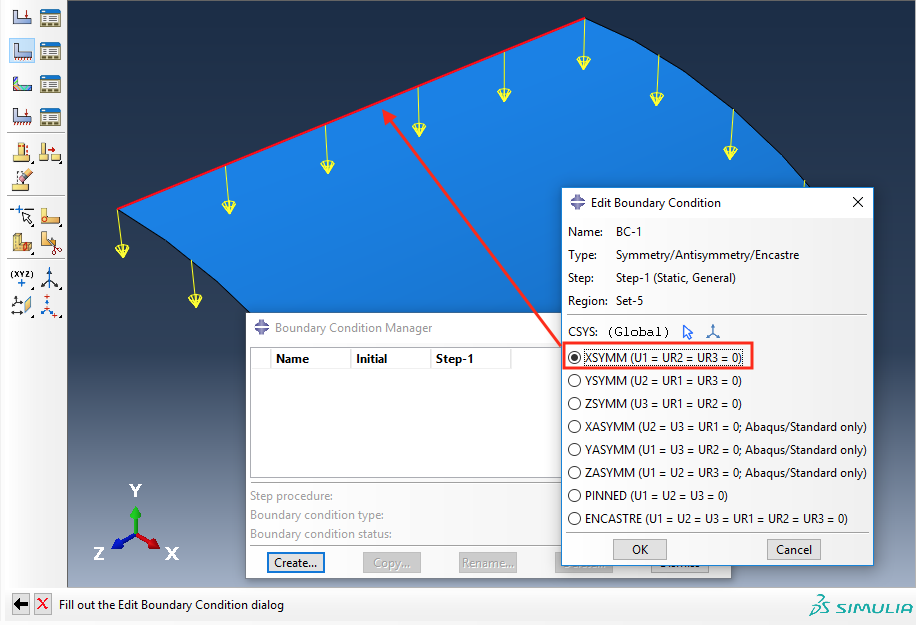
\includegraphics[scale=0.25]{capturas/25-load-x.png}}
\subfigure[Symmetry XSYMM created]{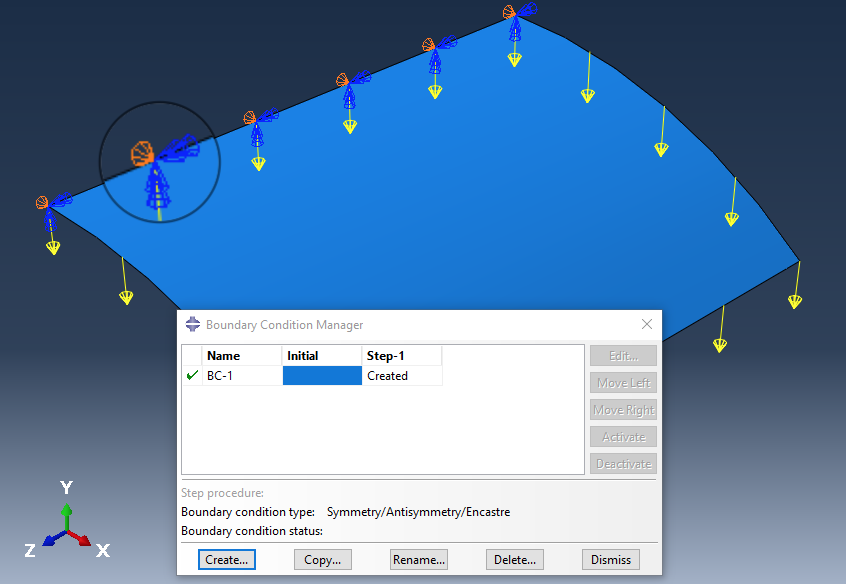
\includegraphics[scale=0.25]{capturas/26-load-x.png}}
\caption{Symmetry boundary conditions ``XSYMM''}
\label{fig:xsymm}
\end{figure}

Establish now the symmetry through plane $z=0$, that is the back side of the model, prescribing the conditions ``ZSYMM'' (Fig.~\ref{fig:zsymm})
%Se establece ahora la simetría por el plano $z=0$, es decir en el borde posterior del modelo, imponiendo las condiciones correspondientes ``ZSYMM'' (Fig.~\ref{fig:zsymm})
\begin{figure}[h!tp]
\centering
\subfigure[Select edge and condition ZSYMM]{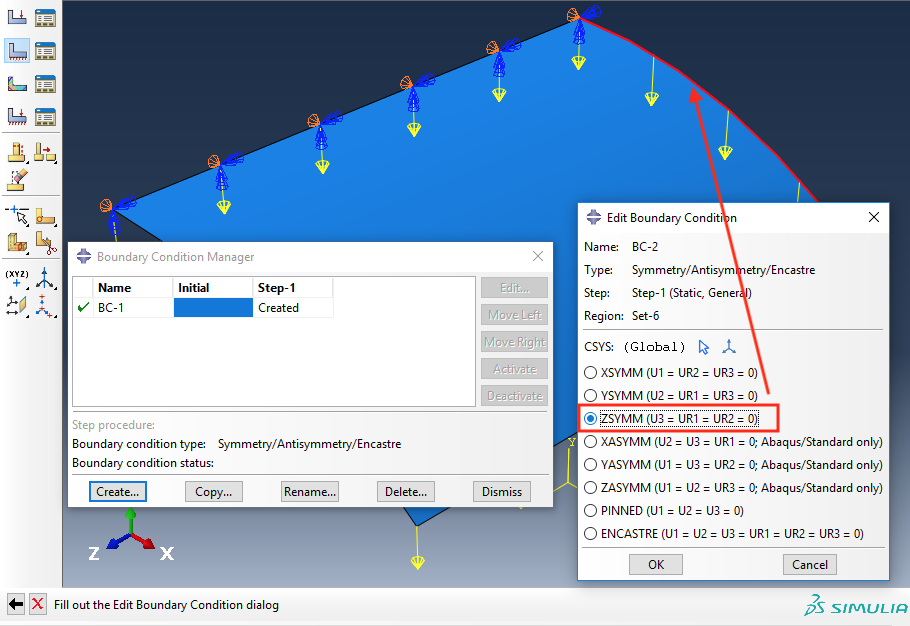
\includegraphics[scale=0.25]{capturas/27a-load-x.png}}
\subfigure[Symmetry ZSYMM created]{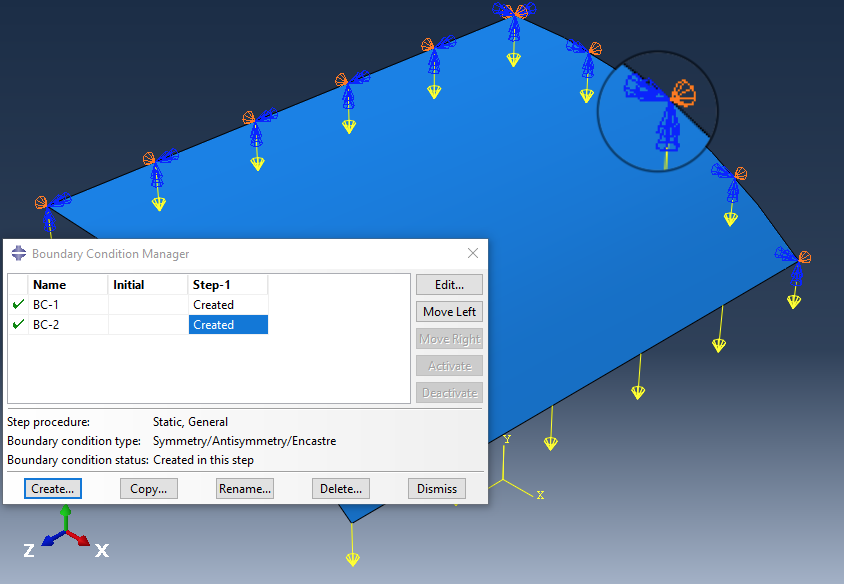
\includegraphics[scale=0.25]{capturas/27b-load-x.png}}
\caption{Symmetry boundary conditions ``ZSYMM'', back edge}
\label{fig:zsymm}
\end{figure}

Finally, in the front edge $z=L/2$, the boundary condition for prescribing the fixed support is created, through conditions of the type \emph{``Displacement/rotation''}, fixing only the degrees of freedom $u_{x}, u_{y}$ (U1 and U2 in Abaqus): (Fig.~\ref{fig:apoyo}).
%Por último, en el borde anterior $z=L/2$, se crea una condición de contorno para imponer el apoyo fijo, mediante condiciones del tipo \emph{``Displacement/rotation''}, fijándose únicamente los grados de libertad $u_{x}, u_{y}$ (U1 y U2 en Abaqus): (Fig.~\ref{fig:apoyo}).
\begin{figure}[h!tp]
\centering
\subfigure[Support in front edge]{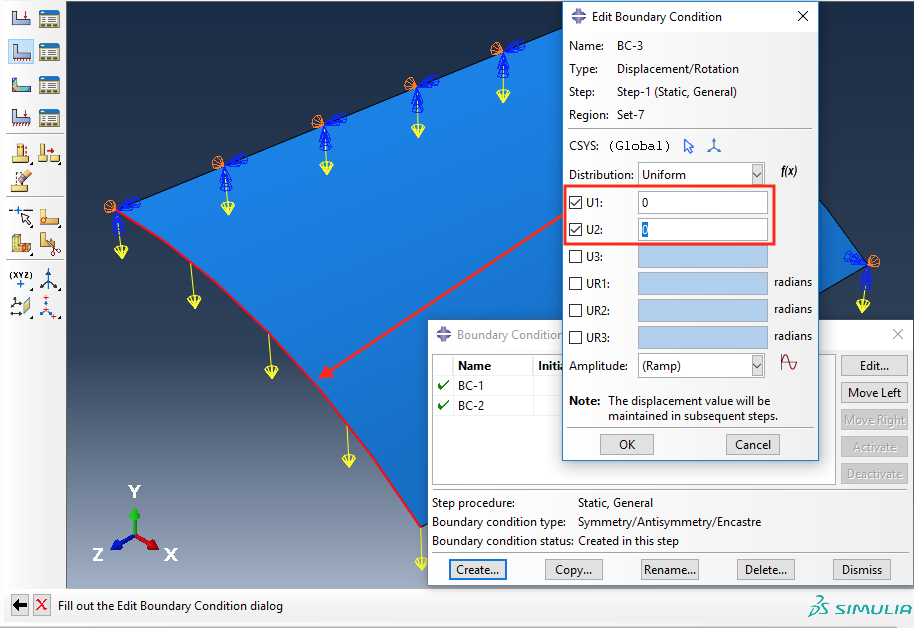
\includegraphics[scale=0.25]{capturas/28b-load-x.png}}
\subfigure[Suppoert and rest of conditions]{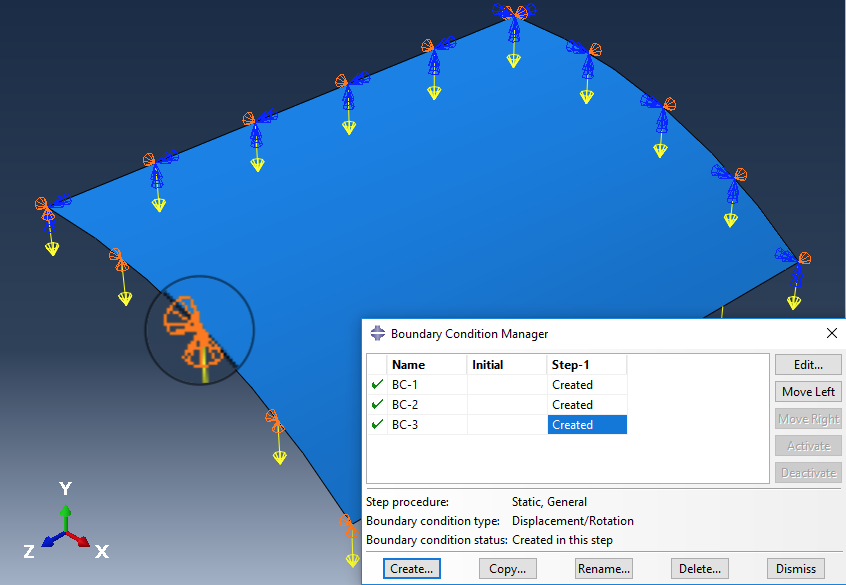
\includegraphics[scale=0.25]{capturas/28c-load-x.png}}
\caption{Boundary conditions for support in the front edge}
\label{fig:apoyo}
\end{figure}
\clearpage

\subsection{\texttt{Mesh} module}

Within the \texttt{Mesh} module, start by selecting the part by expanding the tee of the model at the left side, and activating with the right button the icon \emph{``Mesh''}:
%En el módulo mesh hay que comenzar por seleccionar la parte expandiendo el árbol del modelo / parte de la izquierda, y activando con el botón derecho el icono \emph{``Mesh''}:
Fig.~\ref{fig:mesh-part}.
Open in the top menu bar \emph{Mesh} $\to$ \emph{Controls} and select ``Quad'' and ``Structured'', to generate s structured mesh of quadrilaterals 
%Se abre en el menú superior \emph{Mesh} $\to$ \emph{Controls} y se selecciona ``Quad'' y ``Structured'', para generar una malla estructurada de cuadriláteros
(Fig. \ref{fig:mesh-controls}).
\begin{figure}[h!tp]
\parbox[t]{0.49\textwidth}{%
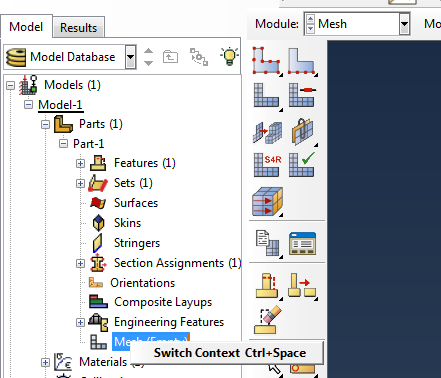
\includegraphics[width=0.5\textwidth]{capturas/29-mesh.png}
\caption{Expanded model tree for mesh.}
%\caption{Seleccionar en el menú desplegado del modelo para mallar.}
\label{fig:mesh-part}%
}\quad
\parbox[t]{0.49\textwidth}{%
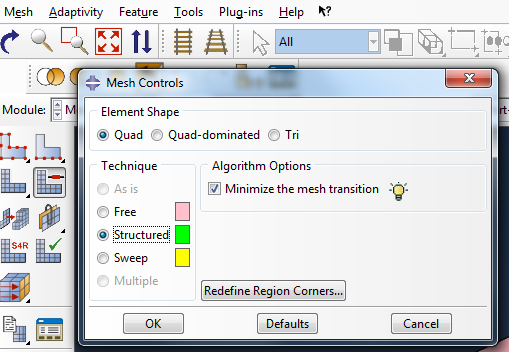
\includegraphics[width=0.5\textwidth]{capturas/30-mesh.png}
\caption{Define options in ``Mesh controls''}
%\caption{Definir opciones en ``Mesh controls''}
\label{fig:mesh-controls}%
}%
\end{figure}

Following, open in the top bar the menu \emph{Mesh} $\to$ \emph{Element type} and select the options \emph{``Shell''}, \emph{``Membrane stress: Small''}, \emph{``Reduced integration''} which will correspond to element type S4R5 
%A continuación se abre en el menú superior \emph{Mesh} $\to$ \emph{Element type} y se seleccionan las opciones ``Shell'', ``Membrane stress: Small'', lo que dará lugar al elemento S4R5
(Fig. \ref{fig:mesh-element}).
\begin{figure}[h!tp]
\centering
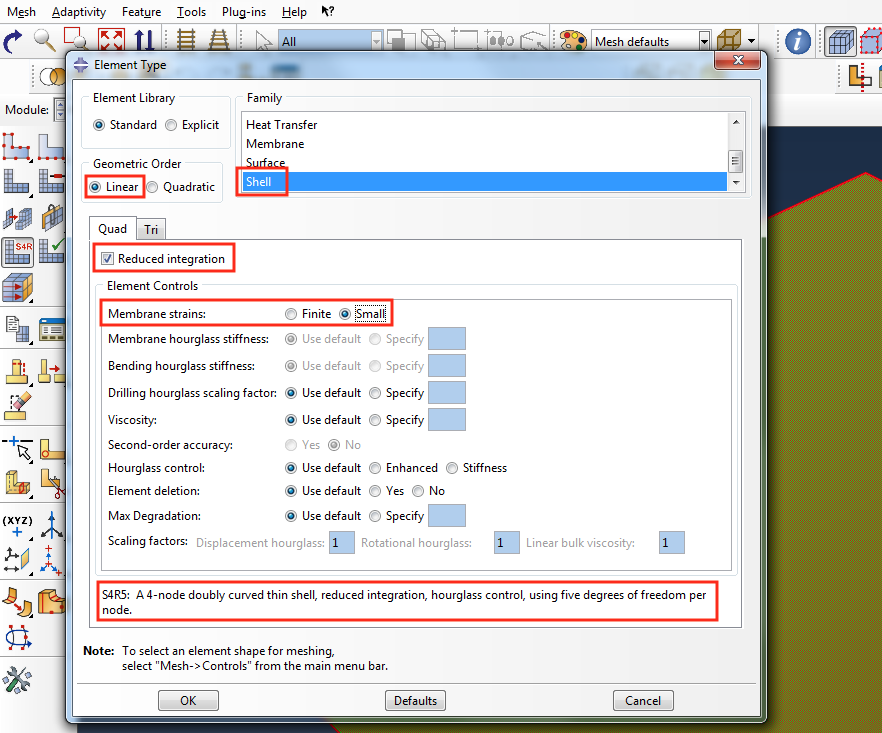
\includegraphics[scale=0.33]{capturas/31-mesh.png}
\caption{Select element type in ``Mesh/element''}
\label{fig:mesh-element}%
\end{figure}

Following the seeds for mesh generation are introduced, this will be done individually for each edge, activating the option ``By number'' and selecting 16 elements per edge. This operation must be performed along two orthogonal edges, in the remaining two it is not required.
%Ahora se introducen las semillas para la generación de la malla, se seleccionan los bordes individuales, se activa la opción ``By number'' y se piden 16 elementos por borde. Esta operación hay que hacerla en dos bordes ortogonales, en los otros dos no es necesario
(Fig. \ref{fig:seeds}).
\begin{figure}[h!tp]
\centering
\subfigure[]{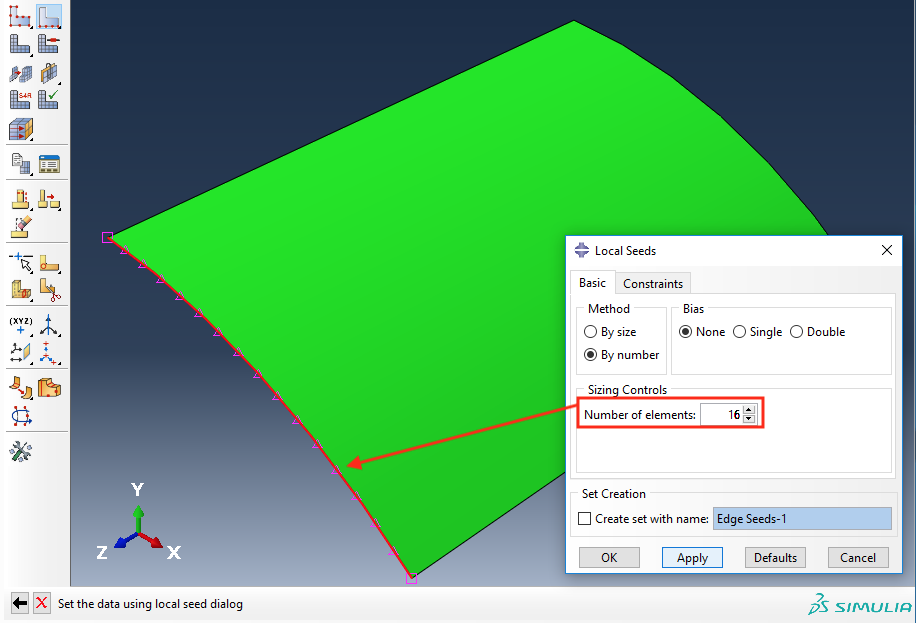
\includegraphics[scale=0.25]{capturas/33a-mesh-x.png}}
\subfigure[]{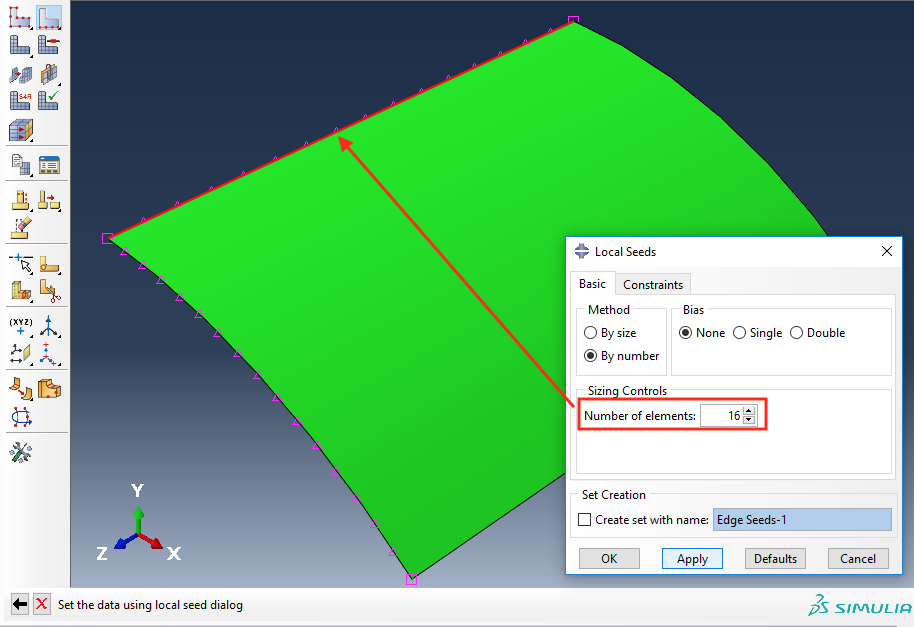
\includegraphics[scale=0.25]{capturas/33b-mesh-x.png}}
\caption{Definition of the number of elements (seeds) on each edge}
\label{fig:seeds}
\end{figure}
Finally mesh the part with the meshing icon indicated in Fig.~\ref{fig:mesh}, obtaining the result shown in the figure.
%Finalmente se malla la parte con el icono de mallado indicado en la figura~\ref{fig:mesh}, obteniéndose el resultado que se muestra.
\begin{figure}[h!tp]
\centering
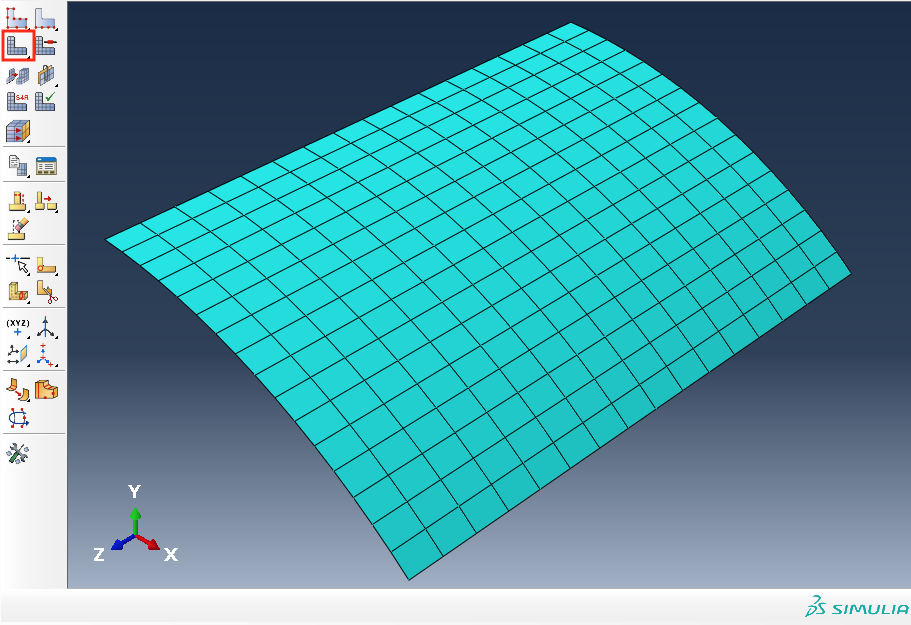
\includegraphics[scale=0.30]{capturas/36-mesh-x.png}
\caption{Meshing of the body}
%\caption{Mallado del cuerpo}
\label{fig:mesh}
\end{figure}

%\clearpage

\subsection{\texttt{Job} module}

Once the model is completed, create a \emph{``Job''} with the default options (Fig.~\ref{fig:job-create}).
%Una vez completado el modelo, se crea un \emph{``Job''} con las opciones por defecto (Fig.~\ref{fig:job-create}).
\begin{figure}[h!tp]
\centering
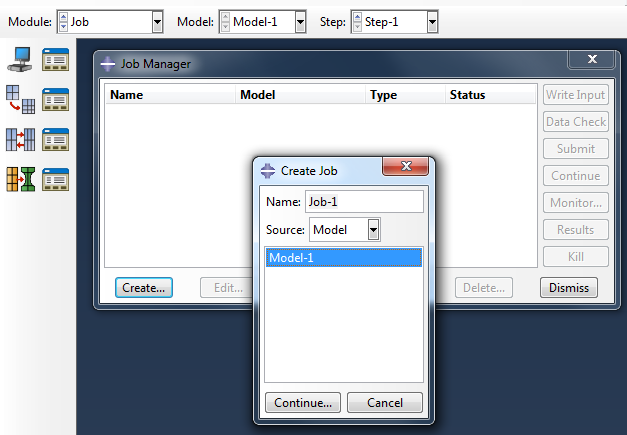
\includegraphics[scale=0.5]{capturas/37-job.png}
\caption{Creation of the \emph{``Job''}}
%\caption{Creación del \emph{``Job''}}
\label{fig:job-create}
\end{figure}

It may now be submitted for calculation through the ``Submit'' button. The \emph{Status} should change from ``Submitted'' $\to$ ``Running'' $\to$ ``Completed''  (Fig.~\ref{fig:job-submit})
%Y se envía para calcular mediante ``Submit''. El \emph{Status} va cambiando de ``Submitted'' $\to$ ``Running'' $\to$ ``Completed''  (Fig.~\ref{fig:job-submit})
\begin{figure}[h!tp]
\centering
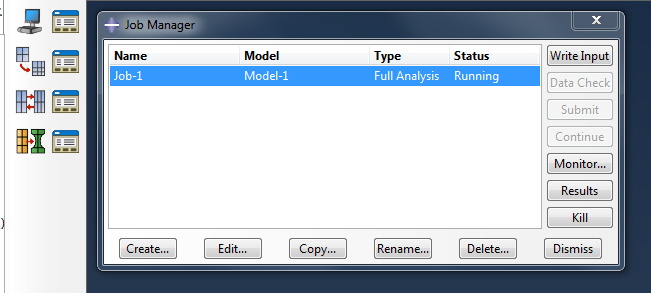
\includegraphics[scale=0.5]{capturas/38-job.png}
\caption{Submission of the ``Job''}
%\caption{Envío del ``Job''}
\label{fig:job-submit}
\end{figure}
If no error message is shown the job is finished and one can enter now the visualization module to view the results, as shown in Fig.~\ref{fig:job-results}.
%Si no hay mensaje de error el problema está acabado y se pasa al módulo de visualizar los resultados, como se muestra en la Fig.~\ref{fig:job-results}.
One may see that the deflection in the middle of the free edge is very close to the reference value $u_{z}=-0.3024$ m.
%Se observa que la flecha en el punto medio del borde libre es muy próxima al valor de referencia  $u_{z}=-0.3024$ m.
%% con la malla 16x16 resulta $u_{z}=-0.3043$ m

Often it is convenient to draw the complete model including the symmetric parts, represented by mirroring views.
%A menudo resulta conveniente representar el modelo completo con las partes simétricas representadas como imagen especular. 
This may be achieved using the menu options ``View'' $\to$ ``ODB display options'', and in the tab ``Mirror / Patterns'' selecting the \emph{Mirror planes} for $XY$ and $YZ$, Fig.~\ref{fig:job-results-symm}.
%Esto se puede obtener mediante las opciones en el menú ``View'' $\to$ ``ODB display options'', escogiendo en la pestaña ``Mirror / Patterns'' los \emph{Mirror planes} para $XY$ e $YZ$, Fig.~\ref{fig:job-results-symm}.
\begin{figure}[h!tp]
\centering
%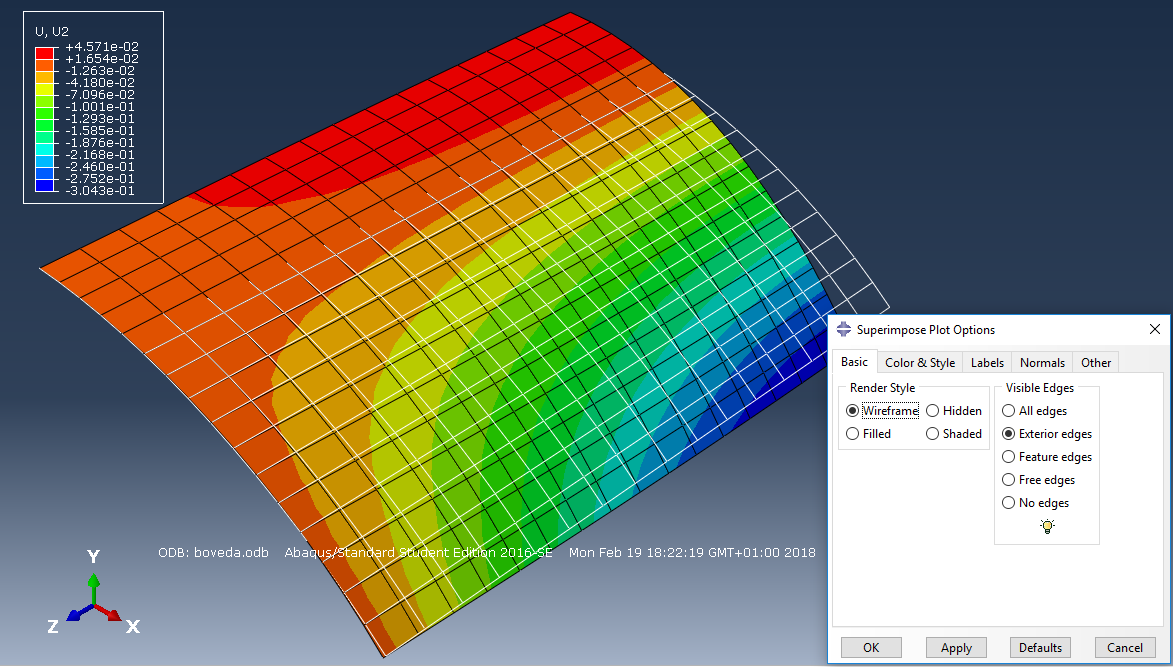
\includegraphics[scale=0.35]{capturas/39-results-U2.png}
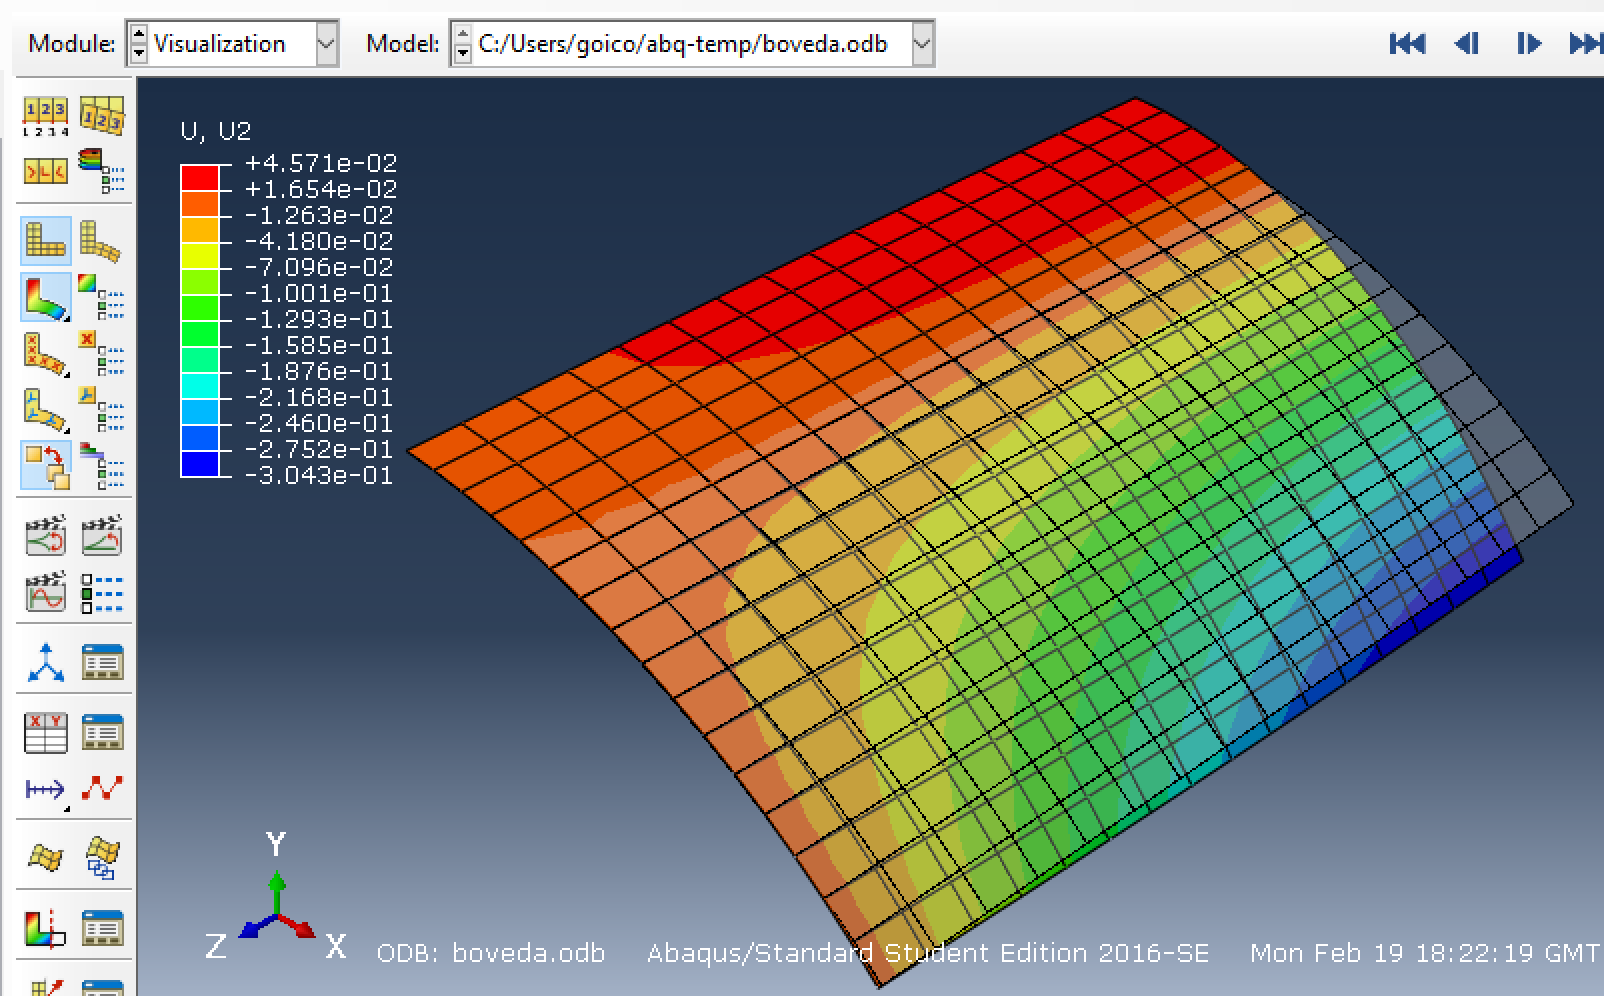
\includegraphics[scale=0.45]{capturas2019/a_fig23.png}
\caption{Results of analysis -- vertical displacement \texttt{U2}}
%\caption{Resultados del cálculo -- desplazamiento vertical \texttt{U2}}
\label{fig:job-results}
\end{figure}
\begin{figure}[h!tp]
\centering
%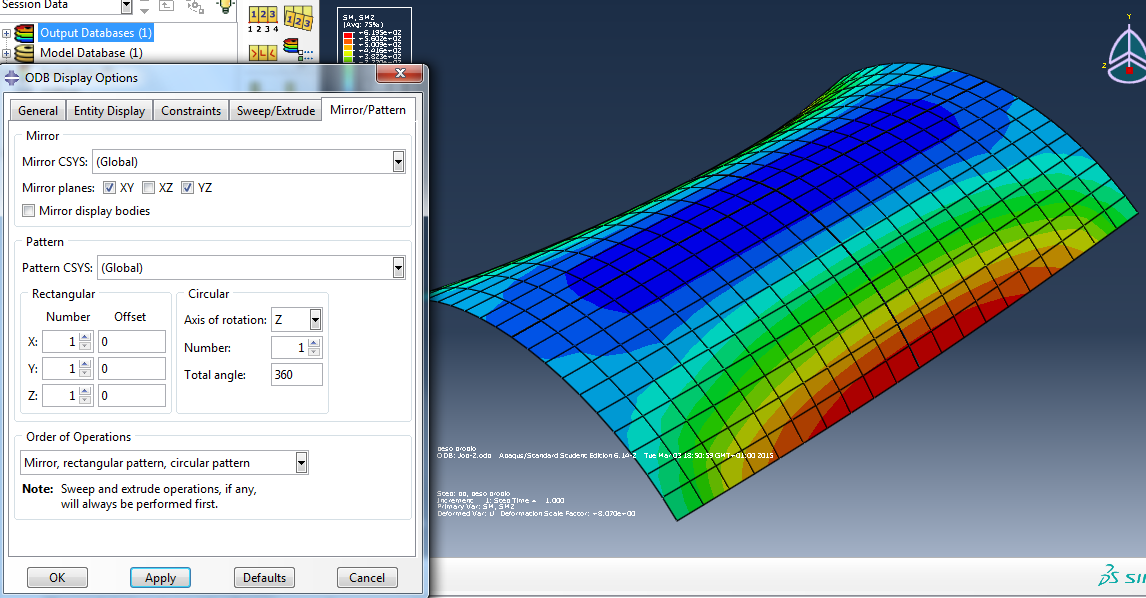
\includegraphics[scale=0.4]{capturas/39a-results.png}
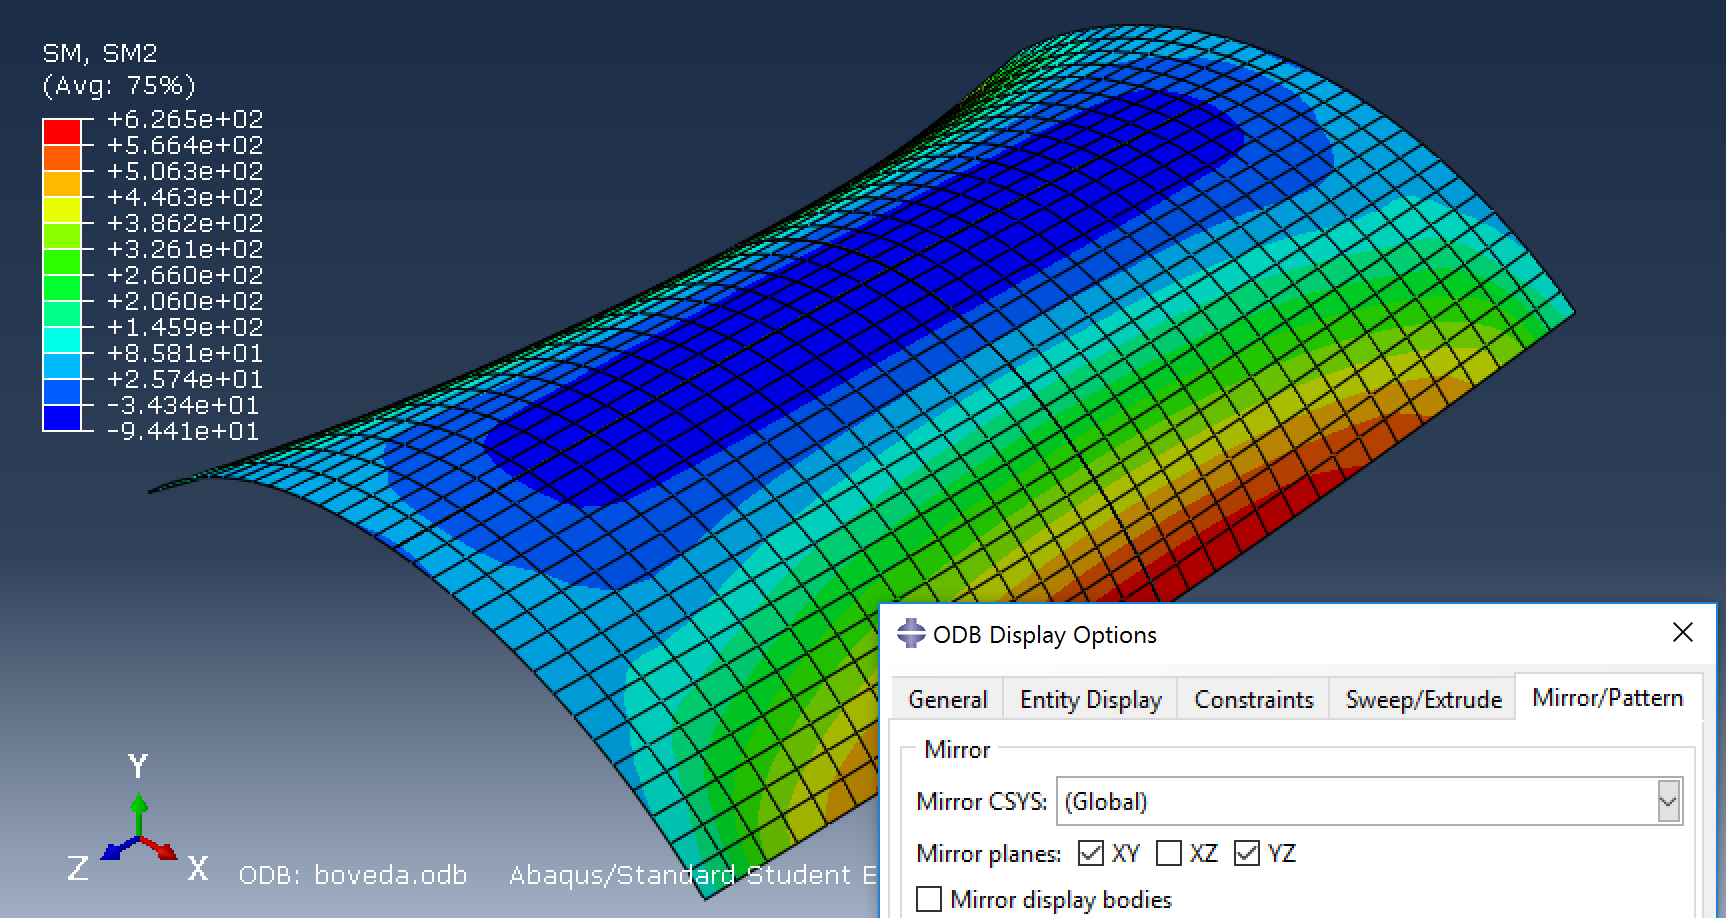
\includegraphics[scale=0.45]{capturas2019/a_fig24p.png}
\caption{View of complete model with symmetric mirror parts included}
%\caption{Vista del modelo completo con las partes simétricas representadas}
\label{fig:job-results-symm}
\end{figure}
\clearpage

\section{Model with continuum elements}
A similar model with continuum elements (3D solids) may be created, following the steps below:
%Se puede crear un modelo similar con elementos de continuo (sólidos 3D), realizando los siguientes pasos:
\paragraph{\S1.---}
Create a part of type ``Deformable'' / ``Solid'' / ``Extrusion'';
%Crear una parte del tipo ``Deformable'' / ``Solid'' / ``Extrusion'';
Define the edges of the part through two circular arches, with respective radii $R_{i}=R-e/2$ y $R_{e}=R+e/2$, spanning the same $40^{\circ}$ as before, and joining later the extremes of both arches to form a closed domain within the plane $XY$.
%Definir el contorno de la parte mediante dos arcos de circunferencia, con radios respectivos $R_{i}=R-e/2$ y $R_{e}=R+e/2$, con los mismos $40^{\circ}$ que antes, y unir posteriormente los extremos de dichos arcos para formar un recinto cerrado en el plano $XY$.
Finish and extrude such section by a distance $L/2=25$ to obtain the 3D geometry of the part, Fig.~\ref{fig:part-solid}.
%Terminar y extruir dicho perfil la distancia $L/2=25$ para obtener la geometría 3D de la parte, Fig.~\ref{fig:part-solid}.
\begin{figure}[h!tp]
\centering
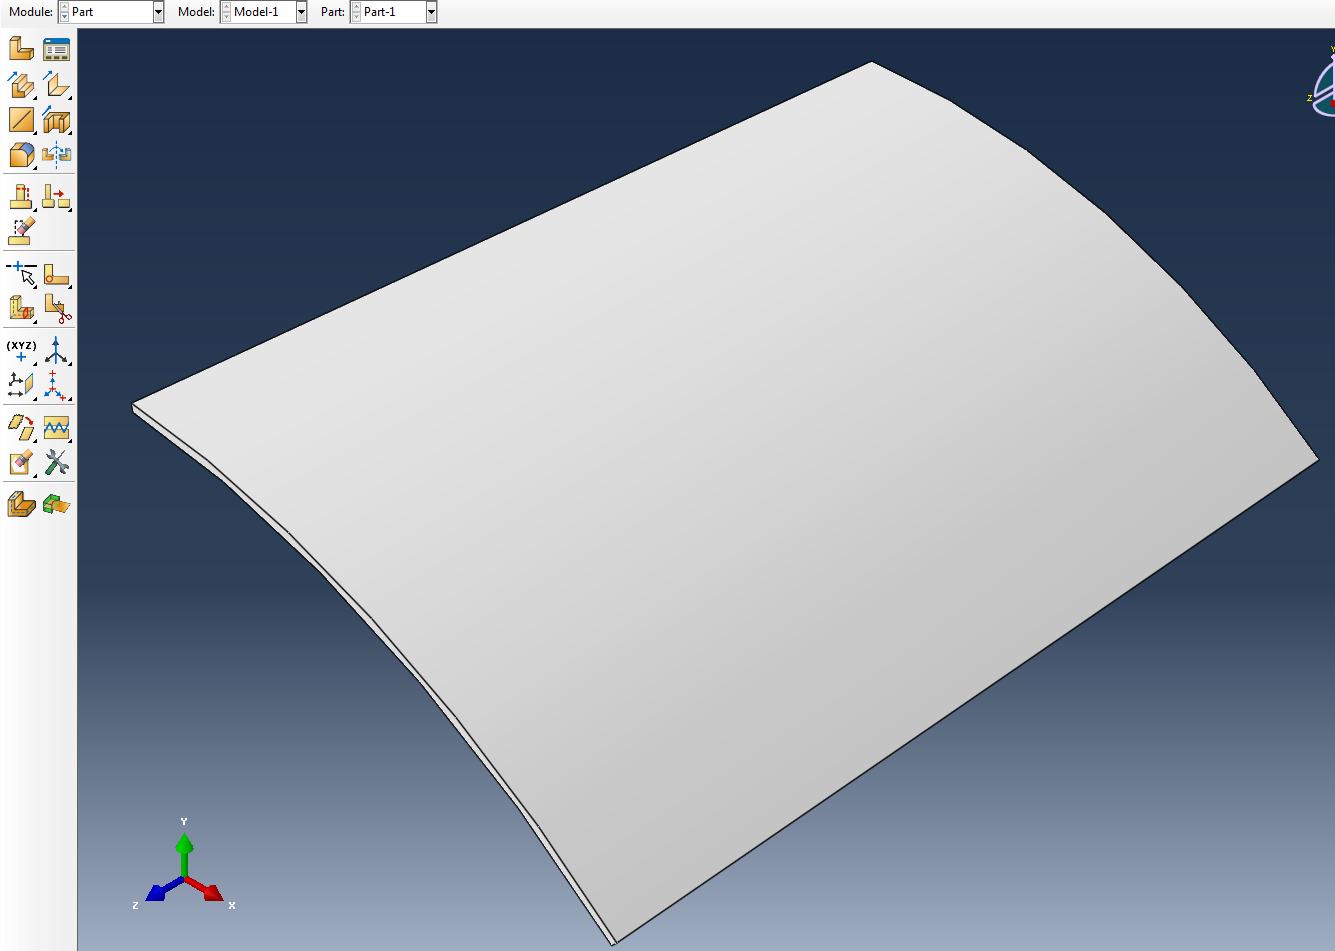
\includegraphics[scale=0.3]{capturas/40-part-solid.png}
\caption{Geometry of the part as a 3D continuum}
%\caption{Geometría de la parte como continuo 3D}
\label{fig:part-solid}
\end{figure}
\paragraph{\S2.---}
In order to define the boundary conditions at the edges be sure to select the complete side, not only one edge, see for instance Fig.~\ref{fig:load-solid} where the symmetry conditions ``ZSYMM'' are specified.
%Para definir las condiciones de contorno en los bordes se debe tener cuidado de seleccionar el borde completo, no solo una arista, ver por ejemplo la Fig.~\ref{fig:load-solid} en la que se definen las condiciones de simetría ``ZSYMM''.
The remaining boundary conditions in the model are established in a similar way.
%El resto de condiciones de contorno en el modelo se establecen de forma similar.
\begin{figure}[h!tp]
\centering
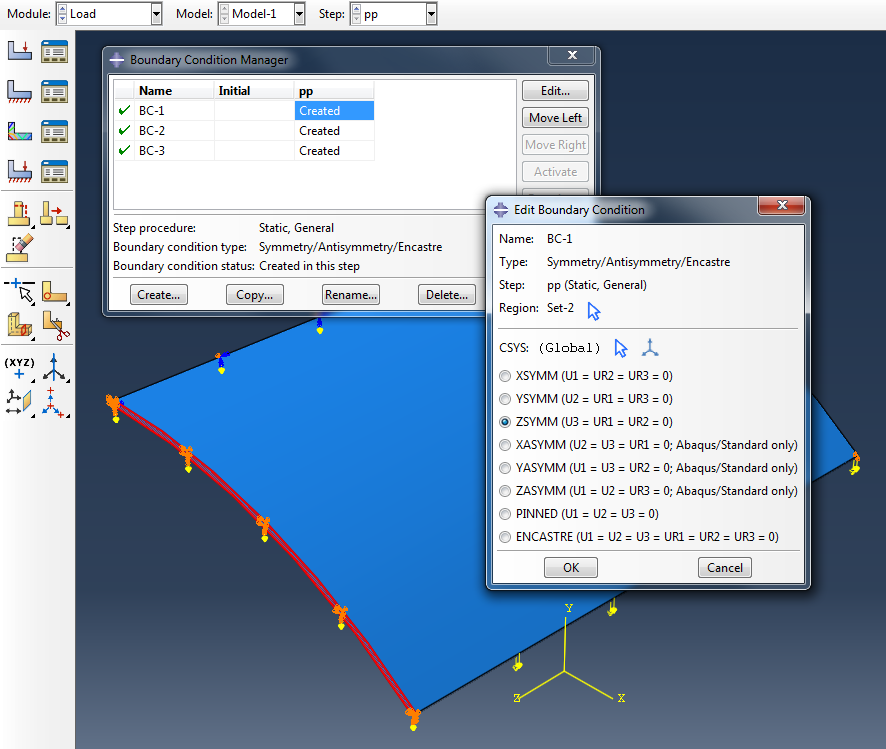
\includegraphics[scale=0.3]{capturas/41-load-solid.png}
\caption{Boundary conditions in the continuum 3D model}
%\caption{Condiciones de contorno en modelo continuo 3D}
\label{fig:load-solid}
\end{figure}
\paragraph{\S3.---}
When selecting the meshing in ``Mesh/controls'' adopt a structured mesh of hexahedra, Fig.~\ref{fig:mesh-c-solid}.
%Para la selección del mallado en ``Mesh/controls'' adoptar una malla estructurada de Hexaedros, Fig.~\ref{fig:mesh-c-solid}.
\paragraph{\S4.---}
For the element type select in the first place the hexahedron with incompatible modes, it is a special element with good results for bending even if there is just one element through the thickness, Fig.~\ref{fig:mesh-e-solid}.
%En el tipo de elemento seleccionamos en primer lugar el hexaedro de modos incompatibles, se trata de un elemento muy especial y que da buenos resultados para flexión a pesar de haber un solo elemento en el espesor, Fig.~\ref{fig:mesh-e-solid}.
\paragraph{\S5.---}
For the meshing, just select the seeds that the system suggests as default options, figure\ref{fig:mesh-s-solid}.
%Para el mallado, basta con seleccionar las semillas que el sistema propone por defecto, Fig.~\ref{fig:mesh-s-solid}. 
The result obtained, with one element through the shell thickness, is shown in Fig.~\ref{fig:mesh-m-solid}.
%El resultado obtenido, con un elemento solo en el espesor de la lámina, se muestra en la Fig.~\ref{fig:mesh-m-solid}. 
\begin{figure}[h!tp]
\parbox[t]{0.39\textwidth}{%
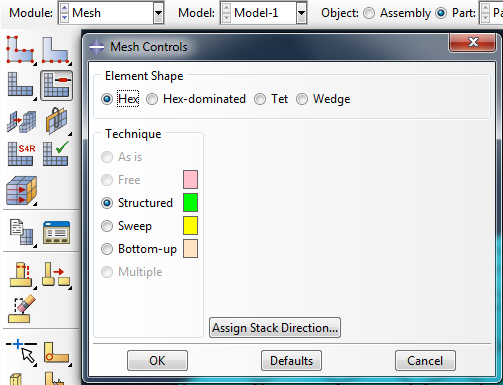
\includegraphics[width=\linewidth]{capturas/42-mesh-solid.png}
\caption{``Mesh / controls'' in continuum 3D model}
%\caption{``Mesh / controls'' en modelo continuo 3D}
\label{fig:mesh-c-solid}
}\quad
\parbox[t]{0.59\textwidth}{%
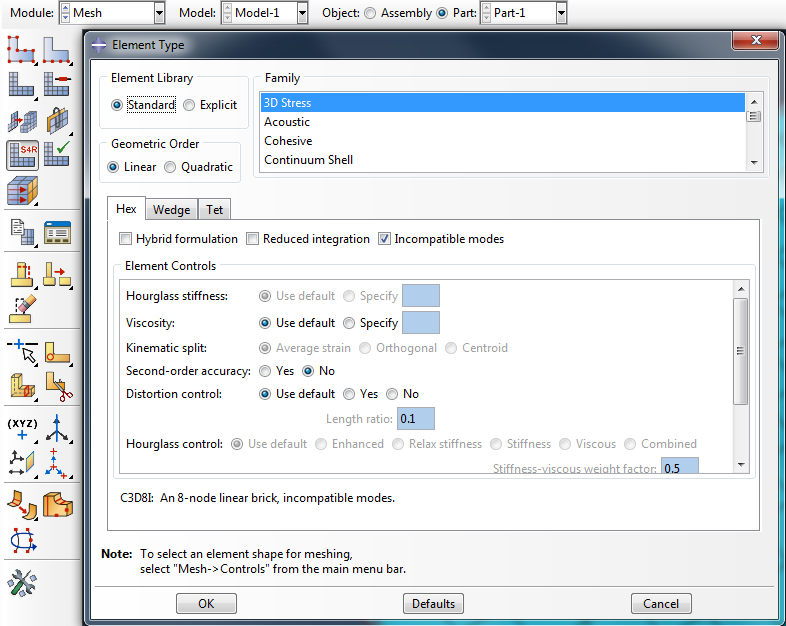
\includegraphics[width=\linewidth]{capturas/43-mesh-solid.png}
\caption{Selection of element type (8 node hexahedron with incompatible modes) within ``Mesh / element type'' for the continuum 3D model}
%\caption{Selección del tipo de elemento (hexaedro de 8 nodos con modos incompatibles) mediante ``Mesh / element type'' en modelo continuo 3D}
\label{fig:mesh-e-solid}
}%
\end{figure}
\begin{figure}[htp]
\centering
\includegraphics[scale=0.5]{capturas/44-mesh-solid.png}
\caption{Seeds for the continuum 3D model}
%\caption{Semillas para el mallado en modelo continuo 3D}
\label{fig:mesh-s-solid}
\end{figure}
\begin{figure}[htb]
\centering
\includegraphics[scale=0.45]{capturas/45-mesh-solid.png}
\caption{mesh of hexahedra for the continuum 3D model}
%\caption{Malla de hexaedros en el modelo continuo 3D}
\label{fig:mesh-m-solid}
\end{figure}

The results obtained with the C3D8I elements are excellent, very similar to those of the shell model.
%Los resultados obtenidos con los elementos C3D8I son excelentes, muy similares a los de elementos lámina. 
The most representative value is the deflection at the centre of the free edge, which is very similar to the reference value $u_{z}=-0.3024$ m.
%La muestra más significativa es la flecha en el centro del borde libre, que resulta ser muy cercana al valor de referencia $u_{z}=-0.3024$ m.
%% en este modelo con 14x19x1 elementos resulta $u_{z}=-0.3032$ m.

If the element type is changed to the standard linear hexahedron with full integration (C3D8) the results are extremely poor, the resulting deflection is now $u_{z}=-0.072$~m.
%Si se modifica el tipo de elemento por el hexaedro lineal estándar con integración completa (C3D8) los resultados son extremadamente malos, la flecha resulta $u_{z}=-0.072$ m.
Finally, selecting the linear hexahedron with reduced integration (C3D8R) the results are also very poor, although not as much as in the previous case, the deflection obtained is now $u_{z}=-0.210$~m.
%Por ultimo, empleando el elemento hexaedro lineal con integración reducida (C3D8I) los resultados son también muy malos, aunque no tanto como en el caso anterior, la flecha resulta $u_{z}=-0.210$ m.
This was to be expected as with the normal element formulation (interpolation) it is not possible to represent the gradient of displacements through the thickness if only one element is taken through the thickness.
%Esto era de esperar ya que con la formulación normal de elementos no es posible representar el gradiente de desplazamientos debido a la flexión si se emplea solo un elemento en el espesor. 
A minimum of 4 to 5 elements through the thickness would be needed, but this would lead to a model with a much higher number of degrees of freedom and consequently more costly.
%Como mínimo serían necesario 4 ó 5 elementos en el espesor, pero esto conduciría a un modelo con un número muy elevado de grados de libertad y muy costoso.
In the case of elements with incompatible modes they represent an exception, within their formulation they include independent strain fields which adapt to the bending deformation and thus represent it correctly.
%El caso de los elementos con modos incompatibles es una excepción, en su formulación incluyen campos de deformaciones independientes que se adaptan y recogen correctamente las deformaciones de flexión. 

\clearpage

%\section{Generación de modelos con scripts \texttt{Python}}
\section{Generation of a model with \texttt{Python} scripts.}

%\subsection{Modelo con elementos lámina}
\subsection{Model with shell element}

Two models are included where directly the models are reproduced thanks to Abaqus CAE.
%Se incluyen dos modelos preparados directamente en python que reproducen los modelos realizados con ayuda de abaqus cae.
Following the scripts are slightly described.
%En lo que sigue se explican someramente las distintas partes de cada script.

The primer model is prepared for the shell element.
%El primer modelo es el preparado para elementos lámina.
It can be downloaded directly from \href{http://stokes.mecanica.upm.es/MCIC_open/practicas/scripts-python/prac3_lamina1.py}{\ttfamily prac3\_lamina1.py}. Once downloaded it can be run directly from Abaqus.
%Se puede descargar directamente en \href{http://stokes.mecanica.upm.es/MCIC_open/practicas/scripts-python/prac3_lamina1.py}{\ttfamily prac3\_lamina1.py}, una vez descargado se puede ejecutar desde abaqus directamente.

In this model, the subsequent stages are followed, describing the points of the sketch of the Fig.~\ref{fig:lamina1}.
\begin{figure}
\centering
%    \includegraphics[width=1.0\textwidth]{imag/im5}
	\includegraphics[scale=0.25]{figs/prac3_lamina1_fig.png}
%  \caption{Nodes and selection}
	%\caption{Croquis para generación de modelo con \texttt{Python} y elementos lámina}
	\caption{Sketch for the generation of the model with \texttt{Python} and shell element }
	\label{fig:lamina1}
\end{figure}

\begin{enumerate}
\item
%Primeramente se define el perfil de la lámina. Esto se hace ayudándose de los puntos que definen el cuarto de lámina que se va a modelar.
First, the profile of the shell is defined, thanks to the points that define the quarter of the shell to be modeled.
%Estos son, el punto $O$ centro de la circunferencia que define la sección transversal de la lámina, $A$ que es el punto de máxima altura de la lámina y que pertenece al plano de simetría longitudinal de la misma y el punto $B$ que pertenece al borde libre. Adicionalmente se define el punto $M$ que se utilizará más adelante.
Point $O$ is the center of the circumference that defines the cross section of the shell. Point $A$ is the one with maximum height which belongs to the longitudinal symmetry plane and point $B$ is the one of the free surface of the same plane. Additionally we define point $M$ that will be employed later. We also define the radius $R$ and the half angle, $ANG$.
%También se definen como variables de python el radio de curvatura de la lámina y el semiángulo (R y ANG).
\item
%Con estos parámetros se definen los puntos en un sistema de coordenadas de dos dimensiones, se crea el arco de circunferencia que define el perfil de la lámina y se realiza la extrusión que genera una parte (p).
With these parameters, the points of the coordinate system in 2D are defined and we can create the circumference arc that defined the profile of the shell and, following, it can be extruded to generate part $P$.
\item
%A continuación se definen el material, la sección (en terminología de abaqus) y la asignación de sección a parte. Obsérvese que para hacer la asignación se usan las  'faces' de la parte de abaqus que representan la superficie ya generada.
Following the material, section and assignment of the section are made. Observe that the assignment of the section employed the faces of the part already created in Abaqus.
\item
%Una vez definido el material y asignado a la parte se genera la instancia a calcular que se denominará 'laminainstancia' y que se almacena en la variable 'myAssembly'. Aquí al generar la instancia se define con malla dependiente de la parte (dependent=ON).
Once defined and assigned the material to the part, the instance is created with the name 'laminainstancia', which is stored in the variable 'myAssembly'. Here, the instance generator is defined with a part dependent mesh property (dependent=ON).
\item
%Posteriormente se definen las cargas y condiciones de contorno. Para seleccionar los elementos geométricos en los que definir las condiciones de contorno nos apoyamos en los puntos medios de los bordes. Con estos puntos medios buscamos el elemento geométrico al que aplica la condición de contorno. En este caso son elementos geométricos del tipo 'edges'. Para esta búsqueda utilizamos puntos definidos en un espacio de tres dimensiones por lo que del punto $M$ definido inicialmente se usan sus dos coordenadas suplementadas por la coordenada $z$ lo que da lugar al punto $OM3$. Para definir el peso propio hay que seleccionar toda la instancia lo que se hace a  mediante un `BoundingBox` de `faces`.
Later loads and boundary conditions are defined. In order to select the geometrical elements where BC are to be defined we take benefit of the middle point of the contours. With these points we look for the geometrical element where the BC is applied. In this case these geometrical elements are of 'edge' type. For this search we employ the defined points in a 3D space, what implies that we need the add the third direction, $z$, to the original defined point $M$, what means the point $OM3$. In order to define the own weight we need to select the whole instance through a `BoundingBox` of `faces`.
\item
%Para definir la malla se generan las divisiones de elementos en dos bordes de la lámina no paralelos, se define el tipo de elemento y se genera la malla.
In order to define the mesh, the divisions of the elements are generated in the two non-parallel contours of the shell. Later, the element type is defined and the mesh can be generated.
\item
%Por último se ejecuta el modelo y se almacena la definición del mismo.
Finally the model is executed and stored its definition.
\end{enumerate}

%\subsection{Modelo con elementos de continuo}
\subsection{Model with solid element}

%El script del modelo con elementos de continuo se puede descargar en \href{http://stokes.mecanica.upm.es/MCIC_open/practicas/scripts-python/prac3_lamina2.py}{\ttfamily prac3\_lamina2.py}. Una vez descargado se puede ejecutar desde abaqus directamente.

The script of the model with solid elements can be downloaded at \href{http://stokes.mecanica.upm.es/MCIC_open/practicas/scripts-python/prac3_lamina2.py}{\ttfamily prac3\_lamina2.py}. Once it is downloaded it can be executed from Abaqus directly.

The programming of this script follows the same patterns of the previous one, with the corresponding exceptions. The points of the sketch of the figure \ref{fig:lamina2} are described.

\begin{figure}
\centering
%    \includegraphics[width=1.0\textwidth]{imag/im5}
	\includegraphics[scale=0.25]{figs/prac3_lamina2_fig.png}
%  \caption{Nodes and selection}
	%\caption{Croquis para generación de modelo con \texttt{Python} y elementos de continuo}
	\caption{Sketch for the generation of the model with \texttt{Python} and solid element }
	\label{fig:lamina2}
\end{figure}
\begin{enumerate}
\item
%Ahora se genera una sección que en vez de estar definida por un tramo de curva abierta se define con una curva cerrada. Los puntos se definen con el siguiente criterio, los puntos pertenecientes a la parte superior de la lámina llevan el sufijo $T$ y los correspondientes a la parte inferior el sufijo $B$.

Now the section is generated with a closed curve instead of an open one. The points are defined with the following criterion: points belonged to the upper part of the shell are defined by the subscript $T$ while the lower ones are written with the subscript $B$.
\item
%La parte se crea mediante una extrusión sólida, BaseSolidExtrude, como contraposición a la lámina que era  BaseShellExtrude.

The part is created through a solid extrusion \textit{BaseSolidExtrude}, opposite to the sell with employs \emph{BaseShellExtrude}.
\item
%La definición del material es similar pero algo más sencilla que en la lámina.

The definition of the material is similar but slightly simpler than for the shell.
\item
%La definición de las cargas se hace utilizando igual que antes puntos medios pero que en este caso en vez de pertenecer a un borde (edge) pertenecen a una  superficie (face). El procedimiento es el mismo que antes, se define el punto medio de la superficie a la que hay que asociar la condición de contorno y se busca la 'face' de la instancia mediante ' findAt'. Para el peso propio se selecciona toda la instancia y para la condición de apoyo se selecciona sólo un borde, en este caso el inferior.

The definition of the loads is made by employing middle points, similarly to the previous case, but in this case these points belong to a face instead to an edge. The procedure is equal to the previous one; the middle point of a surface is defined, a point where the BC is to be associated. The face is find through ' findAt'. For the own weight we can select the whole instance and, for the support, only the lower edge.
\item
%La generación de malla en este caso es con una semilla para todo el modelo.
The generation of the mesh in this case is made with a seed for the whole model.
\item
%El resto del script es similar.
The rest of the script is similar
\end{enumerate}



%\clearpage

\section{Results}
\label{sec:resultados}
\subsection{Deflection at a node}

%\paragraph{Paso 1.} 
The objective is to obtain the deflection in the middle of the free edge, which for the reference model is  $u_{z}=-0.3024$ m.
%Se trata de obtener la flecha en el punto medio del borde libre, que para el modelo de referencia es $u_{z}=-0.3024$ m.
\begin{figure}[h!tp]
%  \begin{center}
%    \subfigure[Tools, query]{\includegraphics[width=0.6\textwidth]{imag/im2_a}}\quad
%    \subfigure[Probe values]{\includegraphics[width=0.25\textwidth]{imag/im3}}
%  \end{center}
\centering
	\subfigure[Tools, query]{\includegraphics[scale=0.50]{capturas2019/a_fig31a.png}}\quad
	\subfigure[Probe values]{\includegraphics[scale=0.50]{capturas2019/a_fig31b.png}}
  \caption{Select values for query of results}
%  \caption{Seleccionar valores a mostrar de los resultados}
  \label{fig2a}
\end{figure}

Using the menu item \emph{tools} (within the results visualisation module), select the submenu \emph{query}  (Fig.~\ref{fig2a}(a)). When opting for this submenu a pop-up window opens in which the option to select is \emph{``Probe values''},
%Se procede utilizando el menú de tools (dentro de resultados) y dentro de tools el submenú query (Fig.~\ref{fig2a}(a)). Al optar por este submenú se abre un recuadro en el que se debe elegir la opción ``Probe values'' (\emph{sondear valores}), 
Fig.~\ref{fig2a}(b).
A new window appears in which one must select \emph{``Probe: Nodes''} and \emph{``Components: Selected''} (Fig.~\ref{fig5}).
%Aparece una nueva ventana en la que se debe elegir ``Probe: Nodes'' y ``Components: Selected'' (Fig.~\ref{fig5}). 
The heading of this window shows the field being viewed, which will be the one probed: \emph{Field output variable for Probe:} U, U2, which may be selected through the icon at the beginning of this field,
%En la cabecera de esta ventana aparece el campo que se está visualizando que será el que se sondee: \emph{Field output variable for Probe:} U, U2, que se puede seleccionar mediante el icono al comienzo de este campo, 
Fig.~\ref{fig7}.
\begin{figure}[h!tp]
\centering
%    \includegraphics[width=1.0\textwidth]{imag/im5}
	\includegraphics[scale=0.45]{capturas2019/a_fig32.png}
  \caption{Nodes and selection}
  \label{fig5}
\end{figure}
\begin{figure}[h!tp]
\centering
%	\includegraphics[width=0.75\textwidth]{imag/im7}
	\includegraphics[scale=0.45]{capturas2019/a_fig33.png}
  \caption{Selection of variable to \emph{probe}: U, U2}
%  \caption{Selección de variable a sondear (\emph{probe}): U, U2}
  \label{fig7}
\end{figure}

Once the desired fields are selected choose with the mouse in the model view window the node or nodes of interest.
%Una vez seleccionados esos campos se debe marcar con el ratón en la ventana de representación del modelo el o los nodos en los que estamos interesados.
When clicking with the mouse on the node the result will be shown in the window \emph{Probe Values}, for this case it happens to be $u_{z}=-0.3043$ m, in agreement with the expected value 
%Al hacer clic con el ratón sobre el nodo en cuestión se verá el resultado en la ventana de \emph{Probe Values} que resulta ser $u_{z}=-0.3043$ m, lo que coincide con el valor esperado 
(Fig.~\ref{fig8}). 
%(Remark: this mesh of $7\times 10$ elements is less refined than the recommended mesh in the exercise ($16\times 16$, due to which the value is slightly less precise.)
%(Nota: esta malla de $7\times 10$ es más grosera que la pedida en el ejercicio ($16\times 16$, por lo que el valor resulta ligeramente distinto, algo menos preciso.)
\begin{figure}[h!tp]
\centering
%	\includegraphics[width=0.95\textwidth]{fm/Fig-1_Despla_Vertical.png}
	\includegraphics[scale=0.45]{capturas2019/a_fig34.png}
%	\includegraphics[width=0.8\textwidth]{imag/im8}
  \caption{Value of deflection (U2) in the selected node}
%  \caption{Valor de flecha (U2) en el nodo seleccionado}
  \label{fig8}
\end{figure}

\clearpage

\subsection{Reaction along an edge}

It is also interesting to obtain the reactions on the supports or on the edges which represent the symmetry conditions.
%Es también interesante obtener las reacciones en los apoyos o en los bordes que representan las condiciones de simetría.
For this one proceeds as in the previous practice, defining a path on the model, in this case it will be the edge of interest.
%Para ello se procede como en la práctica anterior, se define una curva sobre el modelo, en este caso se tratará del borde en el que estemos interesados.
The definition of a path, considering the edges may be curved in general, all the nodes must be included.
%En la definición de la curva, al tratarse de bordes curvos (en general) se deberán incluir todos los nodos que la forman. 
Once the path is defined a table of data is created through the association of a scalar value to the predefined path.
%Una vez definida la curva se define una tabla de datos mediante la asociación de un valor escalar a la curva predefinida.
In this case the procedure is as follows:
%En este caso particular se procedería del siguiente modo:
\begin{enumerate}
\item 
Define the curve
%Se define la curva 
(Fig.~\ref{fig11}). 
This is performed from the tree of results in the left window.
%Ello se hace a partir del árbol de resultados que Fig.~en la  ventana izquierda. 
Select \emph{``Create''} clicking with the right mouse button on the item \emph{``Paths''}.
%Se selecciona \emph{``Create''} haciendo clic con el botón derecho del ratón sobre el item \emph{``Paths''}.
\begin{figure}[h!tp]
\centering
%	\includegraphics[width=0.8\textwidth]{imag/im11}
	\includegraphics[scale=0.45]{capturas2019/a_fig35.png}
%	\includegraphics[scale=0.45]{capturas2019/a_fig35p_fig36a.png}
  \caption{Creation of a path}
%  \caption{Creación de una curva}
  \label{fig11}
\end{figure}
In the next window
%En la ventana siguiente 
(Fig.~\ref{fig13}(a)) 
select  \emph{``Node list''}, give a name to the path and click on \emph{``continue''}.
%se selecciona \emph{``Node list''}, se da un nombre a la curva y se hace clic sobre \emph{``continue''}.
In the next window (Fig.~\ref{fig13}(b)) select \emph{``Add After''} for the creation of the \emph{``Node List''}.
%En la siguiente ventana (Fig.~\ref{fig13}(b)) se indica \emph{``Add After''} para la creación del \emph{``Node List''}.
\begin{figure}[h!tp]
\centering
    \subfigure[Type of path]%
%    \subfigure[Tipo de curva]%
%    {\includegraphics[scale=0.55]{imag/im13}}
    {\includegraphics[scale=0.45]{capturas2019/a_fig36a.png}}
    \quad
    \subfigure[Node List]%
%    {\includegraphics[scale=0.55]{imag/im14}}
	{\includegraphics[scale=0.45]{capturas2019/a_fig36b.png}}
  \caption{Type of curve and list of nodes for definition of the \emph{Path}}
%  \caption{Tipo de curva y lista de nodos para definición del \emph{Path}}
  \label{fig13}
\end{figure}

The nodes are then added,
% as shown in Fig.~\ref{fig15}, 
when all nodes have been completed click on ``Done'',
%(Fig.~\ref{fig18}), 
which will show the window of Fig.~\ref{fig19}, confirm that the path is created, as may be observed in the tree representing the results.
%Se van añadiendo los nodos como se muestra en Fig.~\ref{fig15}, hasta que una vez añadidos todos se hace clic sobre ``Done'' (Fig.~\ref{fig18}), con lo que se muestra la ventana de la figura~\ref{fig19}, se confirma y ya está creada la curva, como se puede observar en el árbol que representa los resultados.
\begin{figure}[h!tp]
\centering
%	\includegraphics[width=0.9\textwidth]{fm/Fig-2_Reacc_Vertical.png}
	\includegraphics[scale=0.45]{capturas2019/a_fig37-2.png}
  \caption{\emph{Path} for the vertical reaction}
%  \caption{\emph{Path} para la Reacción Vertical}
  \label{fig19}
\end{figure}
%\begin{figure}[h!tp]
%  \begin{center}
%    \includegraphics[width=0.9\textwidth]{imag/im15}
%  \end{center}
%  \caption{Definition of nodes in the path}
%%  \caption{Definición de los nodos de la curva}
%  \label{fig15}
%\end{figure}
%\begin{figure}[h!tp]
%  \begin{center}
%    \includegraphics[width=0.9\textwidth]{imag/im18}
%  \end{center}
%  \caption{Path ``Done''}
%  \label{fig18}
%\end{figure}
%\begin{figure}[h!tp]
%  \begin{center}
%    \includegraphics[width=0.4\textwidth]{imag/im19}
%  \end{center}
%  \caption{Path created}
%%  \caption{Curva creada}
%  \label{fig19}
%\end{figure}
\clearpage
\item 
The next step is to associate a result to the path, for which a table is created in a similar way as for the creation of the path.
%El siguiente paso es asociar un resultado a la curva, para lo cual se crea una tabla, de modo similar a la creación de la curva. 
Click on the item \emph{``XYData''} of the tree
%Se hace clic sobre el apartado \emph{``XYData''} del árbol
(Fig.~\ref{fig21}).
\begin{figure}[h!tp]
\centering
%    \includegraphics[width=0.9\textwidth]{imag/im21}
	\includegraphics[scale=0.45]{capturas2019/a_fig38.png}
  \caption{Creation of a table with data}
%  \caption{Creación de una tabla de datos}
  \label{fig21}
\end{figure}
In the following window
%En la siguiente ventana 
(Fig.~\ref{fig22}(b)) 
select the option \emph{``Path''} and continue.
%se elige la opción \emph{``Path''} y se continúa.
After
%Después 
(Fig.~\ref{fig22}(b)) 
The curve indicated in the deployable menu \emph{``Path''} must be associated to the scalar value of interest.
%se asocia a la curva indicada en el menú desplegable de \emph{``Path''} el valor del escalar que nos interese. 
\begin{figure}[h!tp]
\centering
%    \subfigure[\emph{Source}]{\includegraphics[scale=0.45]{imag/im22}}
%    \subfigure[\emph{Data Extraction}]{\includegraphics[scale=0.45]{imag/im24}}
	\subfigure[\emph{Source}]{\includegraphics[scale=0.45]{capturas2019/a_fig39a.png}}
	\quad
	\subfigure[\emph{Data Extraction}]{\includegraphics[scale=0.45]{capturas2019/a_fig39pb.png}}
  \caption{Definition of a \emph{path} for a curve with results}
%  \caption{Definición de la trayectoria (\emph{path}) para una curva de resultados}
  \label{fig22}
\end{figure}
For `\emph{`X Values''} leave the option \emph{``True distance''} and in \emph{``Data Extraction''}, besides selecting the curve, mark \emph{``Undeformed''} and \emph{``Include intersections''}. 
%Para \emph{``X Values''} dejamos la opción de \emph{``True distance''} y en ``Data Extraction'', aparte de elegir la curva, marcamos \emph{``Undeformed''} e \emph{``Include intersections''}. 
For the \emph{``Y Values''} click on the button \emph{``Field Output''} which will provide acceess to the window of
%Para el valor de la ordenada de la curva se hace clic sobre el botón \emph{``Field Output''} con lo que tendremos acceso a la ventana de 
Fig.~\ref{fig26}(a), 
in which one must choose RF, RF2 and then click on \emph{``OK''}.
%en la que elegiremos RF, RF2 y haremos clic sobre \emph{``OK''}. 
It only remains to mark \emph{``Plot''} in the window for data extraction
%Ya sólo queda marcar \emph{``Plot''} en la ventana de Data Extraction 
(Fig.~\ref{fig26}(b)) 
and the graph will be obtained as shown in
%con lo que obtendremos la curva 
Fig.~\ref{fig28}.
\begin{figure}[h!tp]
  \begin{center}
    \subfigure[Component RF2]%
%    {\includegraphics[scale=0.45]{imag/im26}}
	{\includegraphics[scale=0.45]{capturas2019/a_fig40pa.png}}
\quad
    \subfigure[\emph{Data Extraction}: options]%
%    {\includegraphics[scale=0.45]{imag/im27}}
    {\includegraphics[scale=0.45]{capturas2019/a_fig40pb.png}}
  \end{center}
  \caption{Extraction of data to a table}
%  \caption{Extracción de datos a una tabla}
  \label{fig26}
\end{figure}
%\begin{figure}[h!tp]
%  \begin{center}
%    \includegraphics[width=1.0\textwidth]{imag/im28}
%  \end{center}
%  \caption{Vertical reaction at the support}
%%  \caption{Reacción vertical en el apoyo}
%  \label{fig28}
%\end{figure}
\begin{figure}[!htp]
\centering
%\includegraphics[width=0.9\textwidth]{fm/Fig-3_Reacc_Vertical_longitud.png}
\includegraphics[scale=0.35]{capturas2019/a_fig41p2a.png}
\quad
\includegraphics[scale=0.35]{capturas2019/a_fig41p2.png}
\caption{Vertical reaction at the support by unit length}
%\caption{Reacción vertical por unidad de longitud en apoyo}
  \label{fig28}
\end{figure}
\end{enumerate}

Additionally, we can obtain the integral of the reaction force per unit length, selecting in the model tree
\emph{XY Data} $\to$ \emph{Create} $\to$ \emph{Operate on XY data} obtaining the result in figure~\ref{fig:int-reac-vert}.
%Además, se puede obtener la integral de la reacción por unidad de longitud, mediante la selección en el árbol del modelo
%\emph{XY Data} $\to$ \emph{Create} $\to$ \emph{Operate on XY data} $\to$ \emph{integrate}
%obteniendo el resultado de la figura~\ref{fig:int-reac-vert}.
\begin{figure}[!htbp]
\centering
%\includegraphics[width=0.9\textwidth]{fm/Fig-4_Integral_Reacc_Vertical}
\includegraphics[scale=0.45]{capturas2019/a_fig42p.png}
\caption{Integral of the vertical reaction(\emph{Moment} represents the integral)}
%\caption{Integral de la reacción vertical (\emph{Moment} representa la integral)}
\label{fig:int-reac-vert}
\end{figure}
\clearpage

It is interesting to carry out as a check the direct calculation of the total reaction, Fig.~\ref{fig:calc-anal-reac}, which as we see differs slightly (5\%) from the value integrated along the \emph{path}.
The cause is that the option \emph{path} is not the most precise way of computing reactions, as there is an interpolation error.
The most precise way would be to add up the individual reactions of each node, as seen in Fig.~\ref{fig:suma-reac-nod}.
%Es interesante hacer como comprobación los cálculos directos de la reacción total, figura~\ref{fig:calc-anal-reac}, que comprobamos que difiere ligeramente (5\%) del valor integrado en el \emph{path}.
%La razón es que la opción \emph{path} no es la forma más exacta de sumar reacciones ya que hay una interpolación de por medio. 
%La forma más precisa sería sumar las reacciones individuales de cada uno de los nodos, como se aprecia en la figura~\ref{fig:suma-reac-nod}
\begin{figure}[!htbp]
\centering
\includegraphics{fm/Fig-5_Analitico_Reacc_Vertical}
\caption{Direct ``hand'' calculation of reaction}
%\caption{Cálculo analítico de la reacción}
\label{fig:calc-anal-reac}
\end{figure}
\begin{figure}[!htbp]
\centering
%\includegraphics[scale=0.8]{fm/Fig-6_Suma_reacciones.png}
\includegraphics[scale=0.45]{capturas2019/a_fig44p1.png}
\caption{Sum of nodal reactions}
%\caption{Suma de reacciones nodales}
\label{fig:suma-reac-nod}
\end{figure}

Yet a different way to obtain the total reaction without resorting to add them up by hand is to establish a constraint of all the nodes along the edge to a single node through an \emph{MPC} or \emph{kinematic coupling} and recover the reaction on that node.
For this purpose the front edge is coupled through a kinematic constraint to a single node which may be real or fictitious, and to which a fixed boundary condition is assigned.
This way the reaction obtained is that corresponding to the total resultant along the edge.
In this case the master node is one of the corners, Fig.~\ref{fig:asig-kine-coup}.
%Otra forma de obtener la suma de reacciones sin tener que \emph{sumarlas manualmente} es establecer una restricción de todos los nodos  del borde de interés a un único nodo mediante un \emph{MPC} o un \emph{kinematic coupling} y recuperar la reacción en dicho nodo.
%Para ello al borde anterior se acopla una restricción cinemática a un único nodo que puede ser real o ficticio y al que se asigna la condición de contorno fija. 
%De este modo la reacción obtenida es la correspondiente a la resultante total de ese borde. 
%En este caso el nodo maestro es uno de los vértices, figura~\ref{fig:asig-kine-coup}.
\begin{figure}[!htp]
\centering
\includegraphics[width=0.9\textwidth]{fm/Fig-7_Kinematic_constraint.png}
\caption{Assignment of a \emph{kinematic coupling} MPC}
%\caption{Asignación de \emph{kinematic coupling} MPC}
\label{fig:asig-kine-coup}
\end{figure}

The Boundary condition is assigned to the master node, Fig.~\ref{fig:asig-cond-cont}.
%Se asigna la condición de contorno al nodo maestro, figura~\ref{fig:asig-cond-cont}.
\begin{figure}[!htp]
\centering
\includegraphics[width=0.9\textwidth]{fm/Fig-8_BC_Nodo_Maestro.png}
\caption{Assignment of the boundary condition}
%\caption{Asignación condición de contorno}
\label{fig:asig-cond-cont}
\end{figure}

If this procedure is followed the result is exact, as may be appreciated in Fig.~\ref{fig:calc-reak-kinem}.
%Si se hace así el resultado es completamente exacto como se puede apreciar en la figura~\ref{fig:calc-reak-kinem}.
\begin{figure}[!htp]
\centering
\includegraphics[width=0.9\textwidth]{fm/Fig-9_Kinematic_Reacc_Vertical.png}
\caption{Calculation of reaction through a \emph{kinematic coupling}}
%\caption{Cálculo de la reacción mediante \emph{kinematic coupling}}
\label{fig:calc-reak-kinem}
\end{figure}


%\clearpage
\addtocontents{toc}{\protect\vspace{1ex} \protect\hrule}
\mbox{}


\clearpage
\section{Proposed exercise}
%El puente de la Fig.~\ref{figuprop1}, de ancho 3,5 m, se encuentra empotrado en pilas y estribos en las áreas verticales de contacto con el terreno circundante. El módulo de Young del material es de 30.0 GPa, el coeficiente de Poisson es $\nu=0.2$ y el peso específico es $\gamma=24000 \mathrm{~N} / \mathrm{m}^{3}$. Las acciones a considerar serán el peso propio y el efecto de un sismo que se supondrá equivalente a una fuerza volumétrica, distribuida transversalmente al puente, de valor $1000 \mathrm{~N} / \mathrm{m}^{3}$, actuando en el sentido AB (Fig.~\ref{figuprop1}).

The bridge of Fig.~\ref{figuprop1}, with a width of 3,5 m, it is clampled at both sides between piles and abutments and the terrain. The Young  modulus of the material is 30.0 GPa, Poisson is equal to $\nu=0.2$ and the own weight is $\gamma=24000 \mathrm{~N} / \mathrm{m}^{3}$. The loads to consider are the own weight and the effect of a seismic action, which is equivalent to a volumetric force, distributed across the bridge, with a value of $1000 \mathrm{~N} / \mathrm{m}^{3}$,acting in the AB direction (Fig.~\ref{figuprop1}).

%Se desea estudiar el comportamiento estructural de este puente ante las dos acciones mencionadas. Teniendo en cuenta las simetrías del problema, se preparará un modelo con Abaqus de la mitad del puente tal y como se indica en la Fig.~\ref{figuprop1}, donde se detalla la geometría de la estructura.

We want to study the structural behavior of this bridge against the two aforementioned actions. Taking into account the symmetry of the problem, it is necessary to prepare an Abaqus model of the half of the bridge as it is depicted in the Fig.~\ref{figuprop1}, where the geometry of the structure is detailed.

\begin{figure}[!h]
  \begin{center}
    \includegraphics[width=0.55\textwidth]{./figs/prop}
  \end{center}
  \caption{Description of the proposed exercise}
  \label{figuprop1}
\end{figure}

Evaluate the following questions taking into account  that the element to be employed is an hexaedron of 8 nodes with reduced integration C3D8R and the size of the element to employ in Abaqus will be $0.55 \mathrm{~m}$.

%Responde las preguntas que vienen a continuación teniendo en cuenta que el elemento a emplear será el hexaedro de 8 nodos con integración reducida C3D8R y el tamaño del elemento a utilizar en el mallador de Abaqus será $0.55 \mathrm{~m}$.

\begin{enumerate}
%\item Flecha vertical (valor absoluto) en el punto B:
\item Vertical displacement (absolut value) at point B:
  \begin{multicols}{4}
  \mybox{A: $3.1\cdot 10^{-5}$ $m$} 
\columnbreak
\mybox{B: $42.1\cdot 10^{-3}$ $m$}
\columnbreak
\mybox{C: $42.1\cdot 10^{-5}$ $m$} %ok$
\columnbreak
\mybox{D: $3.1\cdot 10^{-3}$ $m$}
  \end{multicols}
%\item Peso total del modelo:
\item Total weight of the model:
  \begin{multicols}{4}
\mybox{A: 0.0679 MN}
\columnbreak
\mybox{B: 0.8148 MN} 
\columnbreak
\mybox{C: 1.0 MN}
\columnbreak
\mybox{D: 1.6296 MN} %ok$
  \end{multicols}
%\item M\'axima tensi\'on de tracci\'on en el modelo:
\item Maximum tensile stress in the model:
  \begin{multicols}{4}
\mybox{A:  $0.09$ MPa}
\columnbreak
\mybox{B: $-1.642$ MPa} 
\columnbreak
\mybox{C: $0.393$ MPa}%ok$
\columnbreak
\mybox{D: $450.6$ MPa}
\end{multicols}
%\item Suma de las reacciones horizontales (direcci\'on AB) del modelo en valor absoluto:
\item Sum of the horizontal reactions (AB direction) of the model (absolut value):
  \begin{multicols}{4}
\mybox{A:  $1629.6$ kN}
\columnbreak
\mybox{B:  $1.0$ kN} 
\columnbreak
\mybox{C: $67.9$ kN}%ok$
\columnbreak
\mybox{D: $0.5$ kN}
\end{multicols}
\item Minimum compression stress at the centroid of element E1:
%\item M\'inima tensi\'on de compresi\'on en el centroide del elemento E1:
  \begin{multicols}{4}
\mybox{A:   $-0.113$ MPa}
\columnbreak
\mybox{B: $0.5$ MPa} 
\columnbreak
\mybox{C: $-1.47$ MPa}%ok$
\columnbreak
\mybox{D:  $0.113$ MPa}
\end{multicols}
%\item Tensi\'on vertical en el punto D:
\item Vertical stress at point D:
  \begin{multicols}{4}
\mybox{A:  $-283.5$ kPa}%ok$
\columnbreak
\mybox{B:  $-3048.4$ kPa} 
\columnbreak
\mybox{C:  $-30.9$ kPa}
\columnbreak
\mybox{D:   $117.9$ kPa}
\end{multicols}
\end{enumerate}


\end{document}
